\documentclass[10pt]{article}
\pdfoutput=1 

\addtolength{\oddsidemargin}{-.875in}
\addtolength{\evensidemargin}{-.875in}
\addtolength{\textwidth}{1.75in}

\addtolength{\topmargin}{-.875in}
\addtolength{\textheight}{1.75in}

\openup 1em

%macro for commenting
\usepackage{color}
\newcommand{\leo}[1]{{\color{blue}{\it leo: #1}}}

\newcommand{\Xbeta}{ X_i \beta}
\newcommand{\xbeta}{ x_i \beta}
\newcommand{\xbetaij}{ x_{ij}^T \beta}
\newcommand{\sgamma}{s_{ij}^T\gamma_i}

\usepackage[round]{natbib}

\usepackage{rotating}
\usepackage{graphicx}
\usepackage{subcaption}

\usepackage{float}


\usepackage{amsthm,amsmath} 
\usepackage{amssymb}
\usepackage{subcaption}

\newtheorem{theorem}{Theorem}
\newtheorem{lemma}{Lemma}
\newtheorem{corollary}{Corollary}
\newtheorem{remark}{Remark}


\usepackage{algorithm}
\usepackage{algpseudocode}

\usepackage{mhequ}
\newcommand{\be}{\begin{equs}}
\newcommand{\ee}{\end{equs}}
\newcommand{\bb}[1]{\mathbb{#1}}
\newcommand{\mc}[1]{\mathcal{#1}}
\DeclareMathOperator{\Binom}{Binomial}
\DeclareMathOperator{\No}{No}
\DeclareMathOperator{\PG}{PG}
\DeclareMathOperator{\Bern}{Bernoulli}
\DeclareMathOperator{\U}{Uniform}
\DeclareMathOperator{\cov}{cov}
\DeclareMathOperator{\var}{var}
\DeclareMathOperator{\diag}{diag}
\DeclareMathOperator{\bigO}{\mc O}
\newcommand{\James}[1]{\textcolor{blue}{#1}}


\thispagestyle{empty}
\baselineskip=28pt

\title
{{Calibrated Data Augmentation for Scalable \\ Markov Chain Monte Carlo}}


\author{
     Leo L. Duan,
     James E. Johndrow,
     David B. Dunson
    % \textsuperscript{*}\footnotemark[2]\and
}

 
\begin{document}
    
\maketitle

% generally I don't use abbreviations in an abstract; some journals don't allow it
{\bf Abstract:} Data augmentation is a common technique for building tuning-free Markov chain Monte Carlo algorithms. Although these algorithms are very popular, 
autocorrelations are often high in large samples, leading to poor computational efficiency.  This phenomenon has been attributed to a discrepancy between Gibbs step sizes and the rate of posterior concentration in large samples.  In this article, we propose a family of calibrated data augmentation algorithms, which adjust for this discrepancy by inflating Gibbs step sizes with an auxiliary parameter. The bias introduced by the scale parameter can be eliminated through a Metropolis-Hastings step, or in some cases, controlled with suitable working parameters. The approach is applicable to a broad variety of existing data augmentation algorithms, and we focus on three popular models: probit, logistic and Poisson log-linear.  Theoretical support is provided and dramatic gains are shown in applications.
\vskip 12pt

%\baselineskip=12pt
%\par\vfill\noindent
% ``scaling limit'' refers to the limiting differential equation that an MCMC algorithm converges to as dimension \to \infty, so I removed that
{\noindent  KEY WORDS:  Bayesian probit; Bayesian logit; Approximate Markov chain Monte Carlo; Big $n$; Data Augmentation; Maximal Correlation; Polya-Gamma.}
%\par\medskip\noindent
%\clearpage\pagebreak\newpage
\pagenumbering{arabic}

\section{Introduction}

With the deluge of data in many modern application areas, there is pressing need for scalable computational algorithms for inference from such data, including uncertainty quantification (UQ).  Somewhat surprisingly, even as the volume of data increases, uncertainty often remains sizable.  Examples in which this phenomenon occurs include financial fraud detection \citep{ngai2011application}, disease mapping \citep{wakefield2007disease} and online click-through tracking \citep{wang2010click}.  Bayesian approaches provide a useful paradigm for quantifying uncertainty in inferences and predictions in these and other settings.

The standard approach to Bayesian posterior computation is Markov chain Monte Carlo (MCMC) and related sampling algorithms. Non-sampling alternatives, such as variational Bayes, tend lack general accuracy guarantees. However, it is well known that conventional MCMC algorithms often scale poorly in problem size and complexity. Due to its sequential nature, the computational cost of MCMC is the product of two factors: the evaluation cost at each sampling iteration and the total number of iterations needed to obtain an acceptably low Monte Carlo error. The latter is related to the properties of the Markov transition kernel; we will refer to this informally as the \emph{mixing properties} of the Markov chain. 

In recent years, a substantial literature has developed focusing on decreasing computational cost per iteration (\cite{minsker2014robust,srivastava2015wasp,conrad2015accelerating} among others), mainly through accelerating or parallelizing the sampling procedures at each iteration. Moreover, myriad strategies for improving mixing have been described in the literature. For Metropolis-Hastings (M-H) algorithms, improving mixing is usually a matter of contructing a better proposal distribution. An important difference between M-H and Gibbs is that one has direct control over step sizes in M-H through choice of the proposal, while Gibbs step sizes are generally not tunable. Thus, improving mixing for Gibbs has historically focused on decreasing autocorrelation by changing the update rule itself, for example by parameter expansion (PX), marginalization, or slice sampling.\footnote{Although strictly speaking, slice sampling is just an alternative approach to sampling from a full conditional distribution, in practice, it is often an alternative to data augmentation, so that using a slice sampling strategy results in the removal of a data augmentation step from an alternative Gibbs sampler.} 

The treatment of the behavior of MCMC for large $n$ and/or $p$ in the theory literature is arguably somewhat limited. Historically, many authors have focused on studying the mixing properties of MCMC by showing a general ergodicity condition, such as the geometric ergodicity condition of (cite Meyn and Tweedie, Roberts and Rosenthal). This generally yields bounds on the convergence rate and spectral gap of the Markov chain under consideration, but \cite{rajaratnam2015mcmc} observe that in many cases, these bounds converge to zero exponentially fast in $p$ or $n$, so that no meaningful guarantee of performance for large problem sizes is provided by most existing bounds. In the probability literature, a series of papers have developed an analogue of Harris' theorem and ergodic theory for infinite-dimensional state spaces (cite Hairer, Mattingly and friends papers). Recent work verifies the existence of MCMC algorithms for computation in differential equation models with dimension-independent spectral gap (Hairer, Stuart, Vollmer). In this example, the algorithm under consideration is a M-H algorithm, and it is clear that the proposal must be tuned very carefully to achieve dimension independence. Other work has studied the properties of the limiting differential equation that describes infinite-dimensional dynamics of MCMC.

A recent paper (\cite{johndrow2016inefficiency}) studies the popular data augmentation algorithms for posterior computation in probit, \citep{albert1993bayesian} and logistic models \citep{polson2013bayesian}, showing that the algorithm fails to mix in large sample sizes when the data are imbalanced. An important insight is that the performance can be largely explained by a discrepancy between the rate at which Gibbs step sizes and the width of the high-probability region of the posterior converge to zero as the sample size increases. Thus, since Gibbs step sizes are generally not tunable, slow mixing is likely to occur as the sample size grows unless the order of the step size happens to match the order of the posterior width. This implies that if a way to directly control the step sizes of the Gibbs sampler could be devised, it would be possible to make the mixing properties of the sampler insensitive to sample size by scaling the step sizes appropriately. This is similar to the conclusion of (HSV), except in this case, we have growing $n$ instead of growing $p$, and the Markov chain under consideration evolves according to a Gibbs sampler instead of M-H.

In this article, we propose a method for tuning Gibbs step sizes by introducing auxiliary parameters that change the variance of full conditional distributions for one or more parameters. Although we focus on data augmentation algorithms for logit, probit, and poisson log-linear models, in principle the strategy can be applied more generally to align Gibbs step sizes with the size of the space being explored. In some cases, these ``calibrated'' data augmentation samplers leave the invariant measure unchanged. In other cases, the invariant measure is altered, in which case one can use the Gibbs step as an efficient M-H proposal, thereby recovering the correct invariant, or view the resulting algorithm as a perturbation of the original Markov chain. If the latter strategy is taken, we suggest bias correction through a second set of working parameters. Some theoretical support for the bias-corrected algorithms is provided in terms of bounds on approximation error to full conditionals. 

\section{Calibrated Data Augmentation}
The method is developed primarily in the context of Data augmentation Gibbs samples, which take the general form
\be \label{eq:da}
z \mid \theta, y &\sim p(z;\theta,y) \\
\theta \mid z,y &\sim N(\mu(z),\Sigma(z)),
\ee
thereby allowing conditionally Gaussian updates for the frequently high-dimensional parameter $\theta$. As such, data augmentation is an important computational strategy when the difficulty of tuning Metropolis-Hastings algorithms is prohibitive due to dimension or complexity of the target distribution. An important class of data augmentation algorithms are those for generalized linear models (GLMs) with $\bb E[y_i \mid x_i, \theta] = g^{-1}(x_i \theta)$ and conditionally Gaussian prior on $\theta$. We focus in particular on poisson log-linear, binomial logistic, and binomial probit as motivating examples.

The calibration of step sizes is best illustrated by an example. Consider the binomial probit, with sampling model
\be
y_i \sim \Bern(p_i), \quad p_i = \Phi(x_i \beta),
\ee
and improper prior $\pi(\beta)=1$. The basic data augmentation algorithm (tanner and wong, albert and chib, etc) has the update rule
\be
z_i \mid \beta, x_i, y_i &\sim \left\{ \begin{array}{cc} \No_{[0,\infty)}(x_i \beta,1) & \text{ if } y_i = 1 \\ \No_{(-\infty,0]}(x_i \beta,1) & \text{ if } y_i = 0 \end{array} \right. \\
\beta \mid z, x, y &\sim \No((X'X)^{-1} X'z, (X'X)^{-1}),
\ee
where $\No_{[a,b]}(\mu,\sigma^2)$ is the normal distribution with mean $\mu$ and variance $\sigma^2$ truncated to the interval $[a,b]$. To make the Gibbs step sizes tunable, we introduce an auxiliary parameter $r_i$ as the conditional variance of $z_i$. 
% we can't reset b_i = (\sqrt{r_i}-1) x_i\beta every time, since it won't lead to convergence of Markov chain. instead, we have to fix b_i at some point, leading to different target distribution that needs to be corrected.
To reduce the bias caused by $r_i$, we adjust the mean by another auxiliary parameter $b_i$, giving

\be
\int_{-\infty}^{0} \frac{1}{\sqrt{2 \pi r_i} } \exp\left(-\frac{(z_i-\xbeta-b_i)^2}{2 r_i^2} \right) dz_i = \Phi( \frac{\xbeta+b_i}{\sqrt{r_i}}),
\label{eq:prop-marginal-probit}
\ee
yielding the update rule 
\be
z_i \mid \beta, x_i, y_i &\sim \left\{ \begin{array}{cc} \No_{[0,\infty)}(x_i \beta+b_i,r_i) & \text{ if } y_i = 1 \\ \No_{(-\infty,0]}(x_i \beta+b_i,r_i) & \text{ if } y_i = 0 \end{array} \right. \\
\beta^* \mid z, X &\sim \No((X'R^{-1}X)^{-1} X'R^{-1}(z-b), (X'R^{-1}X)^{-1}),
\ee
where $R = \diag(r_1,\ldots,r_n)$, $b = (b_1,\ldots,b_n)'$. Note that, in the parameter expansion algorithms of \cite{liu1999parameter} and \cite{meng1999seeking}, which rescale $\beta$ by $1/\sqrt{r}$ and leads to no change in the conditional variance for $\beta$; we adjust the mean, allowing us to control the variance of the step sizes through the value of $r$.

To correct the difference between the the adjusted  and the original distributions, we take one M-H step based on the marginal likelihood. Generate one uniform random variable $u\sim \U(0,1)$ and accept the new $\beta^*$ if

\be
u < \frac{\prod_i L(\xbeta^*) Q(\beta^* \Rightarrow \beta)}{\prod_i L(\xbeta) Q(\beta \Rightarrow \beta^*)},
\ee
where $L(a)=\Phi(a)^{y_i} (1-\Phi(a))^{(1-y_i)}$ and $Q(\beta^* \Rightarrow \beta)=Q(\beta \Rightarrow \beta^*) = \prod_i \int\pi(\xbeta^*|z_i)\pi(z_i|\xbeta)d z_i$, due to the symmetry.

When the proposal is accepted $\beta_t = \beta^*$, the covariance:
\be
\cov(\beta_t \mid \beta_{t-1}, r,X,z) = (X'R^{-1}X)^{-1} + (X'R^{-1}X)^{-1} X'R^{-1}\cov(z-b | R) R^{-1}X(X'R^{-1}X)^{-1} 
\ee
so that
\be
\diag((X'R^{-1}X)^{-1}) \le \var(\beta_t \mid \beta_{t-1}, r,X,z), \label{eq:varlb-probit}
\ee
where the variance of $\beta_t \mid \beta_{t-1}$ is lower bounded by linear combination of the $r_i$. In the intercept-only model, the variance is bounded by $\left(\sum_i r_i^{-1}\right)^{-1}$ via \eqref{eq:varlb-probit}, $1/n$ times the harmonic mean of the $r_i$. \cite{johndrow2016inefficiency} show that when $\sum_i y_i = 1$ and $r_i = 1$, $\var(\beta_t \mid \beta_{t-1})$ is approximately $n^{-1} \log n$, while the width of the high probability region of the posterior is order $(\log n)^{-1}$, leading to slow mixing. Thus, to achieve step sizes consistent with the width of the space, we need
\be
\left(\sum_i r_i^{-1}\right)^{-1} &\approx (\log n)^{-1} \\
\intertext{ so if $r_i = r$ for all $i$ }
\frac{n}{r} \approx \log n \Rightarrow r \approx \frac{n}{\log n}. 
\ee

To illustrate, consider a simple case with an intercept only, with $\sum_i y_i =1$ and $n=10^4$. We set $r_i=r$ for all $i$. As a rough estimate of the intercept near $-3.7$, we fix $b_i = -3.7 (\sqrt r -1)$ to have the effective probability near $\Phi(-3.7)= 10^{-4}$ in the proposal distribution (later we will show the adaptation for $b_i$ without using prior knowledge). As shown in Figure~\ref{probit_demo_intercept_proposal}, increasing the conditional variance by $r$ leads to substantial decrease of the autocorrelation of $\beta^*$ in the proposal distribution; after the M-H step at each iteration, the proposal is accepted as $\beta$ into the Markov chain (Figure~\ref{probit_demo_intercept_posteriorsample}) with large probability. This M-H step guarantees that the increase in the step size in the conditional variance does not exceed the real gap in the marginal, since $\mbox{var}(\beta)\ge \mbox E \mbox{var}(\beta|z)$. Consistent with the previous calculation, $r= 1000\approx \frac{n}{\log n}$ leads to the near-optimal adjustment of the step size. It is worth noting that $r=1$ in the proposal and with M-H step corresponds to the original \cite{albert1993bayesian} Gibbs sampler and its reversibilized version \citep{fill1991eigenvalue}, respectively. Apparently, they both suffer from extremely slow mixing.


\begin{figure}[H]
 % \centering
  \begin{subfigure}[b]{0.49\textwidth}
 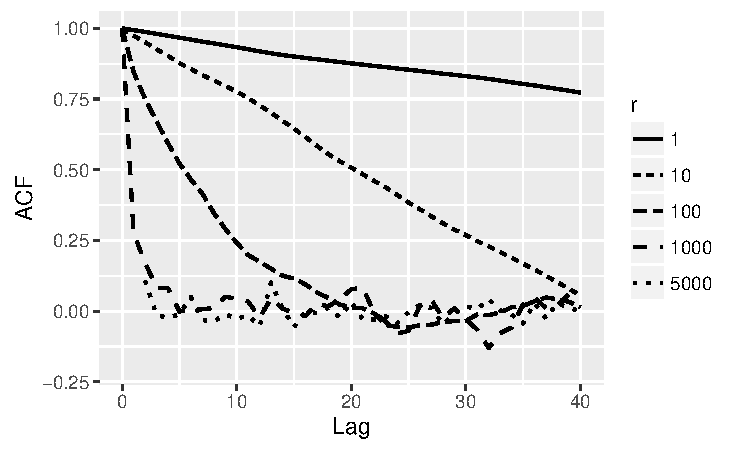
\includegraphics[width=1\textwidth]{probit_demo_acf_prop.pdf}
  \caption{Autocorrelation function (ACF) illustrating the effects of the variance increase of $r$ on improving the mixing of the proposal distribution $\beta^*$.}
 \label{probit_demo_intercept_proposal}
\end{subfigure}
  \hfill
   \begin{subfigure}[b]{0.49\textwidth}
 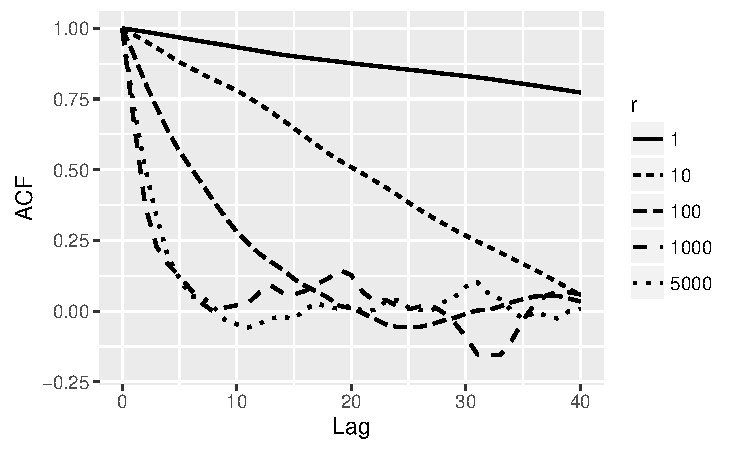
\includegraphics[width=1\textwidth]{probit_demo_acf.pdf}
  \caption{ACF illustrating the mixing of the posterior sample $\beta$ after using Metropolis-Hastings step to accept the proposal from the calibrated distribution.}
   \label{probit_demo_intercept_posteriorsample}
\end{subfigure}
 \caption{Panel (a) demonstrates the adjustment of the step size via increasing the conditional variance in the proposal $\beta^*$ and panel (b) shows its effect after the proposal from the calibrated distribution is accepted as $\beta$ into the Markov chain by the M-H criterion.}
 \label{probit_demo_intercept}
 \end{figure}


\subsection{Adaptation of $r$ and $b$}
Intercept-only probit is a special case where it is possible to estimate the high posterior density region, hence select $b$ and $r$ before sampling. To apply CDA more broadly, we need to be able to handle cases where this condition fails. In this section, we develop a strategy for adaptation of $r$ and $b$.

We set up two sampling periods: first $r$ and $b$ are tuned adaptatively to optimize the acceptance rate; then their values are fixed and the posterior samples are collected.

In the tuning period, we assume $r_i$ is bounded in the region of $[1, \kappa]$, where the lower bound $1$ corresponds to no adjustment and $\kappa$ is a maximal value set to prevent numeric error in the cumulative density function (approximately $5000$ for normal distribution). We start from an moderately large value for all $r_i$. When the step size is large, the proposal distribution is almost free from the mixing problem, but the acceptance rate can be too small if the proposed is out of the high posterior density region; when the step size is small, the acceptance rate is high but the algorithm is inefficient in exploring the region. Note the acceptance rate is the product of  $\alpha_i=\frac{L(x_i \beta^{*})}{L(x_i \beta)}$ over all $i$. When $\alpha_i<1$, we decrease $r_i$ to reduce the step size; when $\alpha_i>1$, we increase $r_i$ to raise the step size. As a heuristic value, we multiply $r_i$ by $\sqrt \alpha_i$ each time. In the meantime, we set $b_i= \xbeta (\sqrt{r_i}-1)$ in each iteration as it minimizes the difference between (\ref{eq:prop-marginal-probit}) and $\Phi(\xbeta)$ given $r_i$ and $\xbeta$.

After the acceptance rate reaches satisfactory level (e.g. $0.3$), we stop tuning and keep $r$ and $b$ fixed. The posterior is collected as ordinary Metropolis-Hastings sampling.

As illustration, we consider regression with an intercept and two predictors $x_{i,1},x_{i,2}\sim \No(1,1)$, with $\beta=\{-5,1,-1\}'$, generating $20$ positive outcomes among $n=10,000$. We apply CDA with initial value of 200 for all $r_i$ and tune the algorithm for 100 iterations, obtaining an acceptance rate of $0.36$.

In this testing case, the \cite{albert1993bayesian} DA algorithm suffers from extremely slow mixing. To compare, we test the parameter expansion algorithm (PX-DA) proposed by \cite{liu1999parameter}. PX-DA reduces the correlation to some extent, however, it does not solve the variance mismatch problem. As shown in Figure~\ref{probit_reg_trace} and \ref{probit_reg_acf}, both DA and PX-DA result in extremely slow mixing. 

In contrast, the calibrated algorithm leads to significant improvement of the mixing (Figure~\ref{probit_reg_trace} and \ref{probit_reg_acf}). In the numerically adapted proposal, the tuned $r_i$ is related to the posterior value of $\xbeta$ (Figure~\ref{probit_reg_r}). The very negative $\xbeta$ ($< -2$) suffers the mis-match in the conditional and marginal variance, hence allows large $r_i$ to adjust the step size. The bias correction is linear in $(\sqrt{r_i}-1 ) \xbeta$ as expected (Figure~\ref{probit_reg_b}).
 
 
\begin{figure}[H]
 % \centering
  \begin{subfigure}[b]{0.49\textwidth}
 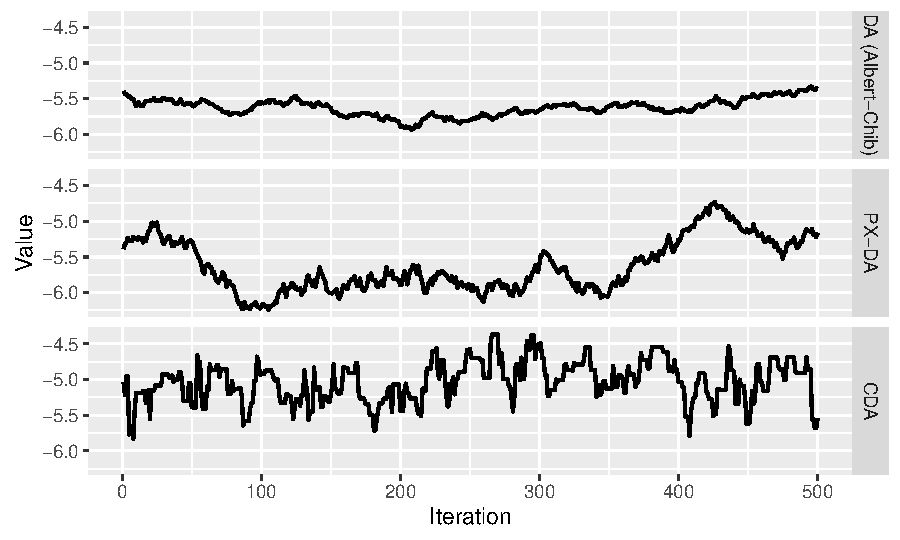
\includegraphics[width=1\textwidth]{probit15_trace_plot.pdf}
  \caption{Traceplot illustrating mixing performance of the original DA, parameter expanded DA and CDA algorithms in probit regression with rare event data.}
  \label{probit_reg_trace}
\end{subfigure}
  \hfill
   \begin{subfigure}[b]{0.49\textwidth}
 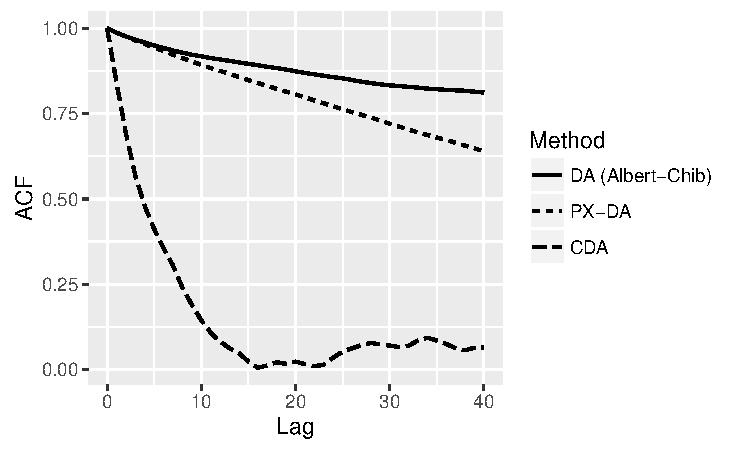
\includegraphics[width=1\textwidth]{probit15_acf.pdf}
  \caption{Autocorrelation function (ACF) illustrating the slow mixing of the DA and parameter expanded DA in rare event data, and CDA correcting this problem.}
    \label{probit_reg_acf}
\end{subfigure}
   \begin{subfigure}[b]{0.49\textwidth}
 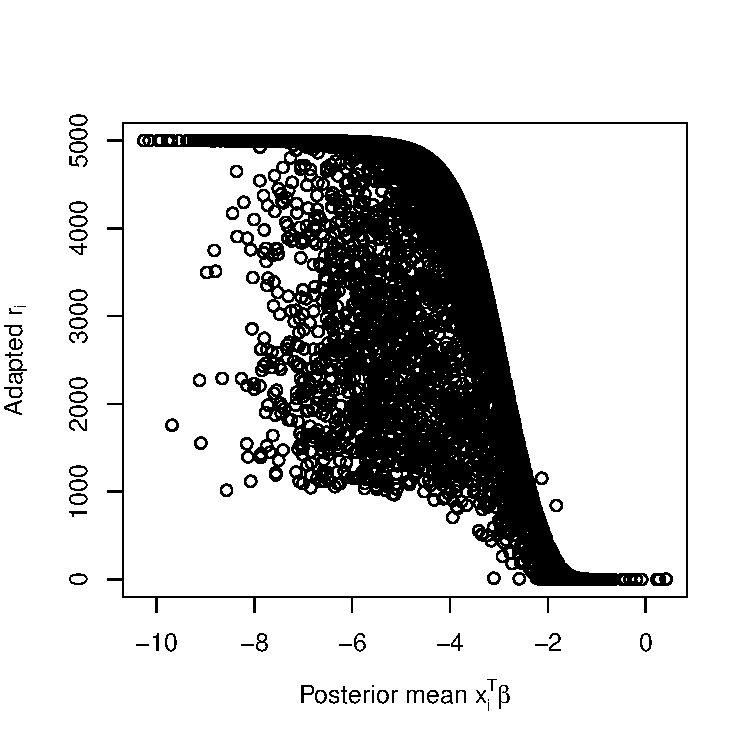
\includegraphics[width=1\textwidth]{probit_cda_r}
  \caption{Numerically adapted $r_i$ showing the room for variance increase is related to the  value of $|\xbeta|$.}
    \label{probit_reg_r}
\end{subfigure}
  \begin{subfigure}[b]{0.49\textwidth}
 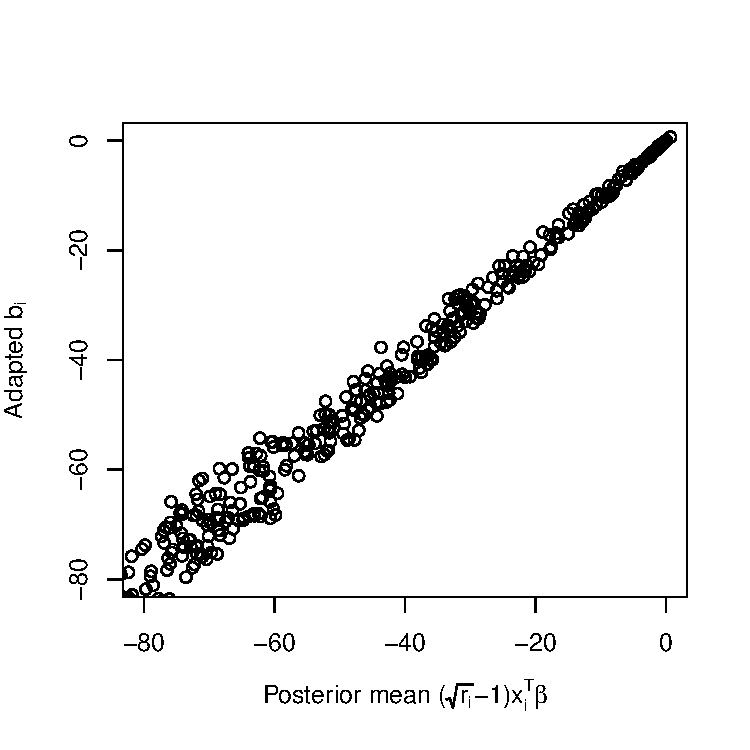
\includegraphics[width=1\textwidth]{probit_cda_b}
  \caption{Numerically adapted $b_i$ learned during the tuning period is close to $(1-\sqrt{r_i} ) \xbeta$ based on the posterior mean.}
      \label{probit_reg_b}
\end{subfigure}
 \caption{Panel (a) demonstrates in traceplot and panel (b) in autocorrelation about the substantial improvement in CDA by correcting the variance mis-match in probit regression with rare event data, compared with the original \citep{albert1993bayesian} and parameter-expanded methods \citep{liu1999parameter}. Panel (c) shows the degree of the variance increase in $r_i$ (if $r_i=1$: no increase) with respect to the value of $\xbeta$. Panel (d) shows the adapted bias correction is close to the true bias baesed on the posterior mean.}
 \end{figure}

\subsection{Alternative Adjustment by Controlling the Latent Variable}

The success of CDA relies on the fact that the calibrated conditional with increased variance can still yield the similar marginal form as the original. Using $\pi(\theta|y)=\int\pi(\theta|z,y)\pi(z|y) dz$, when the variance of $\pi(\theta|z,y)$ does not involve $z$, perturbing it does not affect the integrability. As in the probit example, the original conditional variance for $\beta$ is $(X'X)^{-1}$ and we can multiply $R^{-1}$ in the middle directly. In the other cases, when $z$ is part of the variance, this could pose challenge. Under this scenario, we influence the value of $z$ instead by modifying $\pi(z|y)$.

To illustrate, consider the logistic regression:

\be
y_i \sim \Bern(p_i), \quad p_i = \frac{\exp(x_i \beta)}{1+\exp(x_i \beta)},
\ee
and improper prior $\pi(\beta)=1$. The Polya-Gamma data augmentation has the update rule \citep{polson2013bayesian}:

\be
 z_i &\sim {\PG}(1, |\xbeta|),\\
\beta &\sim \No \left(  (X' Z X)^{-1}   X'  (y-\frac{1}{2})  ,  (X' Z X)^{-1}  \right),
\ee
where $Z= diag(z_1,\ldots,z_n)$. This is due to the integration $L(y_i \mid \xbeta)=  \int \exp\{ \xbeta (y_i-1/2)\} \exp(-\frac{z_i (\xbeta)^2}{2}) \PG(z_i \mid 1,0) dz_i$. Multiplying $r_i$ to $z_i$ would make the integration difficult. Instead, we focus $\PG(z_i \mid 1,0)$ and replace $1$ with the auxiliary parameter $r_i$. Applying bias correction term $b_i$ on $\xbeta$, leading to:


\be
\int_{0}^{\infty}  \exp\{ (\xbeta+b_i) (y_i-r_i/2)\} \exp(-\frac{z_i (\xbeta+b_i)^2}{2}) \PG(z_i \mid r_i,0) dz_i =  \frac{\exp \{ (x_i \beta + b_i)y_i \}}{\{1+\exp(x_i +b_i)\}^{r_i}},
\label{eq:prop-marginal-logit}
\ee
yielding the update rule 

\be
 z_i &\sim {\PG}(r_i, |\xbeta+b_i|),\\
\beta^* &\sim \No \left(  (X' Z X)^{-1}  X'  (y -r_i/2- Zb) ,  (X' Z X)^{-1}  \right),
\ee

Unlike the probit example where the variance increase is deterministic, the step size tuning here is stochastic, based $\bb{E}z_i= \frac{r_i}{2 (|\xbeta+b_i|)}\tanh(\frac{|\xbeta+b_i|}{2})$. With small $r_i<1$, $z_i$ will have small value with high probability, leading to large variance in $(X' Z X)^{-1}$.

Factoring out the constant $\exp(b_i y_i)$ in (\ref{eq:prop-marginal-logit}) and compare with the original density, it can derived the adaptive form for $b_i$ should be $\log[  \{1+\exp(\xbeta)\}^{1/r_i} -1] - \xbeta$. Similar to probit example, M-H step can be used to accept $\beta^*$ if the uniform:

\be
u < \frac{\prod_i L(\xbeta^*) Q(\beta^* \Rightarrow \beta) }{\prod_i L(\xbeta)Q(\beta \Rightarrow \beta^*)},
\ee
where $L(a)=\frac{\exp(a)y_i}{1+\exp(a)}$ and $Q(\beta^* \Rightarrow \beta) =Q(\beta\Rightarrow \beta^* ) $

\subsection{General Algorithm}

Before proceeding into theory, we summarize the general algorithm for CDA. We assume the parameters are multidimensional and divided into two groups $\{ \theta, \eta\}$, where $\theta$ are the ones that suffers from slow mixing. Using Gibbs sampling, we alternatively sample in $\pi(\eta\mid\theta, y)$ and $\pi(\theta\mid \eta,y)$. Omitting $\eta$ for notational ease, using data augmentation form of  $\theta$:

\be \label{eq:da_decomposition}
\pi(f_i(\theta)|y_i) = \int \pi\left(f_i(\theta)|z_i,y_i \right)\pi(z_i|y_i) d z_i
\ee
where $f_i(\theta)$ is the function $f:\bb R^p \mapsto \bb R$, e.g. the individual $x_i\theta$ in regression, and the conditional distribution for $\theta$ is:

\be
\theta \mid z,y &\sim G(\mu,\Sigma).
\ee
We first increase $\Sigma$ by introducing the auxiliary parameter $r_i$: if $\Sigma$ is free from $z$, we modify $\pi\left(f_i(\theta)|z_i,y_i \right)$; otherwise, we change $\pi(z_i|y_i)$. Adding the other parameter $b_i$ to accomodate the bias, we obtain the calibrated data augmentation, integrating to:

\be \label{eq:cda_decomposition}
\pi^{*}(f_i(\theta)+b_i|y_i, r_i) = \int \pi^{*}\left(f_i(\theta)+b_i|z_i,y_i \right)\pi^{*}(z_i|y_i) d z_i
\ee

Then the proposal update rule can be formed:

\be
z_i & \sim \pi(z_i| f(\theta)+b_i) \\
\theta^* &\sim G(\mu^*(f(\theta)+b_i, z),\Sigma^*(z)).
\ee

Using the original likelihood, the individual likelihood ratio can be calculated:
\be
\alpha_i = &\frac{L(f_i(\theta^*))} {L(f_i(\theta))}.
\ee
with the M-H criterion, accepting new $\theta^*$ if the $\U(0,1)$:
\be
u<\frac{ Q(\theta^* \Rightarrow \theta)} {Q(\theta \Rightarrow \theta^*)} \prod_i \alpha_i .
\ee

In tuning period, we start from an $r_i$ that corresponds to moderate increase in the step size. Then at the end of each iteration, increase or decrease $r_i$ based on $\alpha_i>1$ or $\alpha_i<1$ (assuming smaller $r_i$ has larger chance of $\alpha_i>1$); and update $b_i$ to the value that makes $\pi^{*}(f_i(\theta)+b_i|y_i, r_i) = \pi(f_i(\theta)|y_i)$. After the acceptance reaches the preset threshold (e.g. $30\%$), stop adaptation and run MCMC as usual.


\subsection{Special Case without Metropolis-Hastings}

In some cases, if the distance between the proposal $\pi^{*}(f_i(\theta)+b_i \mid y_i, r_i)$ and original $\pi(f_i(\theta)\mid y_i)$ can be strictly bounded, the Metropolis-Hastings step can be skipped, directly accepting $\theta^*$. This generates an approximate Gibbs sampler, a non-reversible Markov chain with a modified target distribution. But since the error is non-noticeable, it can be used as a good and fast approximate to the original slow algorithm.

Taking the logit CDA as an example, note the value for $b_i$ to correct the difference would be $\log[  \{1+\exp(\xbeta)\}^{1/r_i} -1] - \xbeta$. Its expansion yields $\log\{ 1/r_{i} + \frac{1/r_{i}(1/r_{i}-1)}{2!} \exp(\xbeta)+ \frac{1/r_{i}(1/r_{i}-1)(1/r_{i}-2)}{3!} \exp(2\xbeta) +\ldots \ \}$. The suggests when $\exp(\xbeta)$ is close to $0$, $b_i \approx -\log r_{i}$. Then the bound can be calculated between the marginal likelihoods based on the original and calibrated form. We postpone the details of total variation distance to the next section.

This simplifies the update rule to:

\be
 z_i &\sim {\PG}(r_i, |\xbeta - \log r_i|),\\
\beta &\sim \No \left(  (X' Z X)^{-1}  X'  (y -r_i/2- Z \log r) ,  (X' Z X)^{-1}, \right)
\ee
where $r_i$ is taking a small value when $\exp(\xbeta) < \eta$, otherwise $r_i=1$. 

As the posterior are directly generated from the approximate, the bound needs to be carefully controlled via $r_i$. Therefore, instead of  being fixed after the tuning as in the general case, $r_i$ is used adaptively throughout the sampling. This would cause convergence issue; however, choosing $r_{i} = \sup[\tau{\exp(2\xbeta)}  \vee {\exp(\xbeta)} ]  \wedge 1$ ($\tau>1$) as the maximal function of posterior samples leads to a diminishing adaptation scenario: the probability of $r_i$ changing converges to $0$ hence the difference in two consecutive transition kernels diminishes,  ensuring the convergence of the chain \citep{roberts2007coupling}.

For illustration, we use $\beta=\{-9,1\}$ as the intercept and the slope to $x_1\sim \mathcal{N}(0,1)$, $n= 10^5$. This setting leads to rare positive outcome $\sum y_{ij} = 50 $. The different mixing performances in the original DA and the calibrated one are shown in Figure~\ref{logit_random_mixing}.



\begin{figure}[H]
 % \centering
  \begin{subfigure}[b]{0.49\textwidth}
 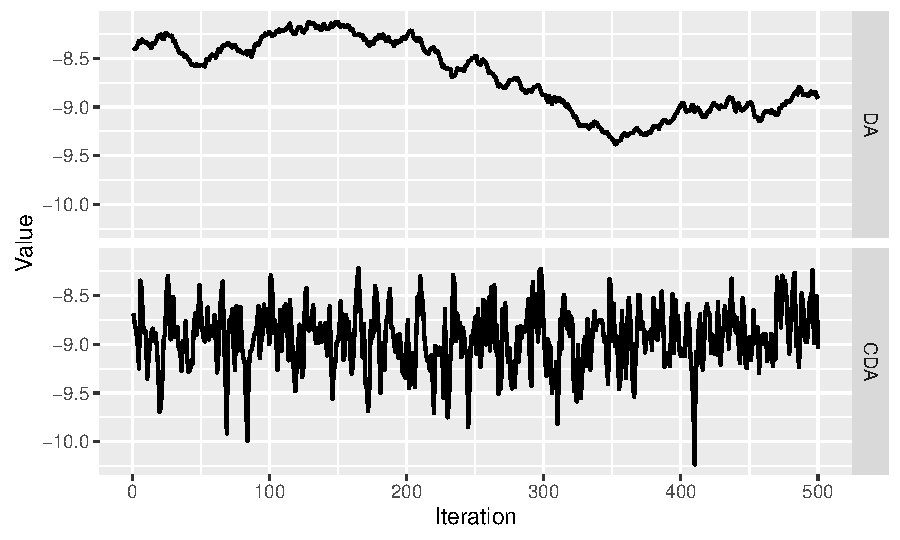
\includegraphics[width=1\textwidth]{logit_random_trace_plot.pdf}
  \caption{Traceplot illustrating mixing performance of the original DA and CDA algorithms in logistic regression.}
\end{subfigure}
  \hfill
   \begin{subfigure}[b]{0.49\textwidth}
 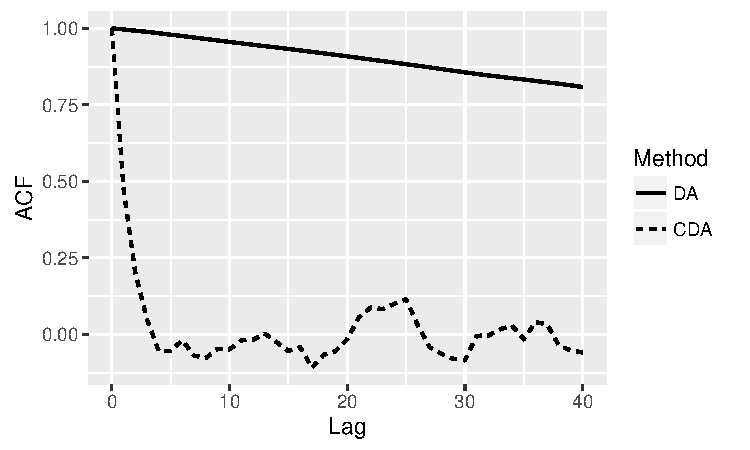
\includegraphics[width=1\textwidth]{logit_random_acf.pdf}
  \caption{Autocorrelation function (ACF) illustrating the large difference between the mixing performance of the original DA and CDA.}
\end{subfigure}
 \caption{Panel (a) demonstrates in traceplot and panel (b) in autocorrelation about the substantial improvement in CDA by correcting the variance mis-match in logistic regression with rare event data, compared with the original \citep{polson2013bayesian}.}
    \label{logit_random_mixing}
 \end{figure}
 
\section{Theory}

\subsection{Mixing Accelaration}

The mixing of Markov chain is related to its geometric convergence rate. Let $\mathcal{P}(\theta,.)$ be the the Markov transition kernel and $\pi(.)$ be its stationary density and $\theta$ be the state in the state space $\varTheta$. The chain is geometrically ergodic if there exist $M: \mathcal{X} \rightarrow [0, \infty)$ and $\rho\in[0,1)$ such that $||\mathcal{P}^k(\theta,.)-\pi(.) ||_{TV} \le M(\theta^{(0)}) \rho^k$, where $||.||_{TV}$ is the total variation distance $|| P_1 -P_2 ||_{TV} = \underset{\mathcal A\in \mathcal F}\sup ||P_1(\mathcal A)-P_2(\mathcal A)||$.

Consider a Hilbert space $L^2(\pi)=\{s(\theta): E\{s(\theta)\}=0, var\{s(\theta)\}<\infty \}$. The forward operator $\bf{F}$ can be defined as ${\bf F}s(\theta)=\int \mathcal{P}(\theta,\theta') s(\theta') d\theta' = E\{ s(\theta') | \theta \}$, whose norm is equal to the maximal correlation between two states $||{\bf F}||=\underset{s(\theta),t(\theta)\in L^2(\pi)}{\sup}\;\mbox{corr}(s(\theta),t(\theta^{'}))$ \citep{liu2008monte}. This norm is directly related to the convergence rate $\rho$: when the chain is reversible with detailed balance (e.g. Metropolis-Hastings), $\lim_{k\rightarrow \infty}||{\bf F}^k||^{1/k}=\rho$; when the chain is non-reversible (e.g. Gibbs sampling), $||{\bf F}||^2$ is equal to the convergence rate of the reversibilized chain \citep{fill1991eigenvalue}.

The two calibrating strategies proposed in the last section reduce the operator norm.

\begin{theorem}
Let ${\bf F}$ and ${\bf F}_{MS}$ be the operators corresponding to the standard DA and the calibrated DA modified with marginalization and sampling (MS), then $||{\bf F}_{MS}||\le ||{\bf F}||$.
\end{theorem}


\begin{theorem}
Let ${\bf F}$ and ${\bf F}_{IV}$ be the operators corresponding to the standard DA and the calibrated DA modified with increased variance (IV). If the relative difference in marginal variance $\frac{|\mbox{var}\{s(\theta)|y  \} - \mbox{var}_{IV}\{s(\theta)|y\} |}{\mbox{var}\{s(\theta)|y \} }\le \epsilon$ and the variance increase $\frac{ var_{IV}\{ \theta|z,y\}}{ var\{ \theta|z,y\}} \ge (1+\epsilon) $, then $||{\bf F}_{IV}||\le ||{\bf F}||$.
\end{theorem}

\subsection{Error Control in Approximate CDA}

For approximate CDA with increased variance, the error needs to be carefully controlled. One can bound the total variation distance $||{P}-{P}_{r,b} ||_{TV}$, where ${P}$ and ${P}_{r,b}$ are the measures for the stationary distributions corresponding to the exact and approximate algorithms. From this bound, one can control the errors of the posterior mean and variance.

\begin{theorem}
Let $\theta$ be the $p$-element vector of $\{\theta_j\}_{j=1\ldots p}$.
If the total variation distance between the two measures defined as above is small $||{P}- {P}_{r,b} ||_{TV}\le \epsilon_1$, $\pi(\theta|y)$ and $\pi_{r,b}(\theta|y)$ have the tail square integral negligible when $|\theta|>M$,  $E \theta_j^2 {1}_{|\theta_j|>M}\le \epsilon_2$ and $E_{r} \theta_j^2 {1}_{|\theta_j|>M}\le \epsilon_2$. Let $M$ be large enough so that $\epsilon_2=o(\epsilon_1)$, then the approximation errors between the first two central moments of $\theta_j$ have:
$$|\mbox{E}(\theta_j|y)-\mbox{E}_{r,b}(\theta_j|y)|\le 2M\epsilon_1+ o(\epsilon_1),$$
$$|\mbox{var}(\theta_j|y)-\mbox{var}_{r,b}(\theta_j|y)|\le 6M^2\epsilon_1+o(\epsilon_1).$$
\end{theorem}
 
 \begin{remark}
 	The assumption on the tail is guaranteed by the existence of the second moment, which implies uniform integrablity. The bound on the variance difference is particularly useful in guaranteeing the average increased conditional variable could at most exceed the target variance by a small error $E^z\mbox{var}_{r,b}(\theta_j|z,y)\le\mbox{var}(\theta_j|y)+\epsilon$, with $\epsilon$ as a polynomial function of $\epsilon_1$ defined as above.
 \end{remark}
 
 The approximation error for the covariance can be similarly bounded:

\begin{corollary}
If $||{P}- {P}_{r,b} ||_{TV}\le \epsilon_1$ and $\pi(\theta|y)$ and $\pi_{r,b}(\theta|y)$, $E \theta_j^2 {1}_{|\theta_j|>M_j}\le \epsilon_2$ and $E_{r,b} \theta_j^2 {1}_{|\theta_j|>M_j}\le \epsilon_2$ for all $j$.  Let $M_j$ be large enough so that $\epsilon_2=o(\epsilon_1)$, then the approximation error between the covariances:
$$|\mbox{cov}(\theta_{j_1},\theta_{j_2}|y)-\mbox{cov}_{r,b}(\theta_{j_1},\theta_{j_2}|y)|\le 6M_{j_1}M_{j_2}\epsilon_1+o(\epsilon_1 ).$$
\end{corollary}

As a special case, we consider in generalized linear model where the total likelihood can be broken into $L(y| B\theta) = \prod  L( y_{i}| B_i^T \theta)$. Here the linear part $B_i^T \theta$ is set in general sense, which could be the combination of both fixed and random effects. Rather than controlling the total distance between $L(y| B\theta)$ and $L_{r,b}(y| B\theta)$, under some  mild conditions of the predictor matrix $B$, one can focus on bounding the maximum error in individual $B_i^T \theta$, based on $ L( y_{i}| B_i^T \theta)$ over $i=1\ldots n$.

\begin{theorem}
If $B^TB$ is full rank and let $B^{-}:=(B^TB)^{-1}B^T$, the following inequalities hold:\\
$$||{E}\theta-{E}\theta_{r,b}||_1 \le ||B^{-}||_1 ||{E}B\theta- {E}B\theta_{r,b}||_\infty$$
$$||\mbox{cov}\theta-\mbox{cov}\theta_{r,b}||_1 \le ||B^{-}||_1 ||B^{-}||_\infty ||\mbox{cov} B\theta- \mbox{cov}B\theta_{r,b}||_\infty$$
\end{theorem}

 \begin{remark}
One reason for using these inequalities is that the norms $||B^{-}||_1$ and $||B^{-}||_\infty$ are usually quite small compared to $n$.  For example, a well-conditioned matrix has $||B^{-}||_\infty\approx p/n$ and $||B^{-}||_1\approx p$.
 \end{remark}

We return to examine the approximate CDA for mixed effects logistic regression, and determined the suitable range for $r_{ij}$.

{\bf Calibration Example 3 (continued): Mixed Effects Logistic Regression}

In the CDA for mixed effects logistic regression, the effective approximate likelihood is $L_{r,b}(y_{ij}|\eta_{ij}) = \frac{\Gamma(1/r_{ij}+1)}{\Gamma(y_{ij}+1)\Gamma(1/r_{ij}-y_{ij}+1)}\frac{\exp (\eta_{ij}+ \log r_{ij})^ {y_{ij}}}{\{1+\exp (\eta_{ij}+ \log r_{ij})\}^{1/r_{ij}}}$. The distance between the approximate and the true likelihoods for each $i$ has $|| { P_{r,b}(y_{ij}|\eta_{ij}) } - {P(y_{ij}|\eta_{ij})} )||_{TV} \le   \{   \frac{\sqrt{r_{ij}-1}  \exp(\eta_{ij})}{2} \} 1 \{\eta_{ij}< - \log r_{ij} \le 0 \}$. The tail square integral $E \eta^2_i 1(|\eta_{ij}|>M) = O\{ M^2 \exp(-M)\}$. Given a maximally tolerable approximation error $\epsilon=0.01$, the calculation leads to  $r_{ij} \le  [\{\frac{10^{-3} }{\exp(\eta_{ij})}\}^2  \wedge {\exp(-\eta_{ij})} ]  \vee 1$. This suggests to apply calibration when $\eta_{ij}< -6.9$ approximately, which is consistent with the rare event scenario.

\subsection{Ergodicity}

The conditions for ergodicity should be met for Markov chains. In the CDA based on marginalization, obviously as long the original chain is ergodic, so is the marginalized chain is, due to its smaller norm of the forward operator. For the CDA based on variance increase, the adaption of the working parameters could influence the ergodicity. In the numeric method, we stop adaption after the tuning period; in the approximate solution, we rely on the the results from \cite{roberts2007coupling} that an adaptive Markov chain is uniformly ergodic, if (i) the transition kernel corresponding to each $r$ is uniformly ergodicity (simultaneous convergence) and (ii) the total variation distance between kernels in two adjacent steps converges to $0$ in probability (diminishing adaptation).

The first condition is simple to achieve since the approximation does not alter the distribution of the transition kernel but only with different parameterization, the condition can be met with only slight modification. For the diminishing adaptation, since $r$ is adapted so that $\sup_{\theta \in \varTheta^*} d(\theta, \theta_{r,b})\le \epsilon$ over the posterior sample $\varTheta^*$, the suitable $r$ could be the extreme function of the posterior $\theta$. When it is true, the convergence of the extreme function in probability leads to the convergence of the transition kernel.

{\bf Calibration Example 3 (continued): Mixed Effects Logistic Regression}

In the CDA with mixed effects logistic regression, we set $r_{ij} =  1 \vee \underset{\eta_{ij}: \theta\in \varTheta^*}{\inf}[\{\frac{10^{-3} }{\exp(\eta_{ij})}\}^2  \wedge {\exp(-\eta_{ij})} ]   $, which is related to the maximum of $\eta_{ij}=\xbeta+s_{ij}\gamma_i$ if $\eta_{ij}<0$. With finite posterior variance of $\beta$ and $\gamma_i$, the value is convergent in probability via Chebyshev's inequality. The diminishing adaption for the numeric example is shown in Figure~\ref{diminishing_adapt}.

 \begin{figure}[H]
 \centering
 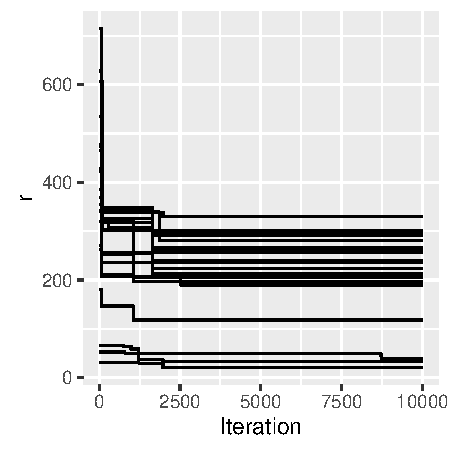
\includegraphics[width=0.3\textwidth]{r_adaptation.pdf}
  \caption{The diminishing adaptation of the working parameter $r_{ij}$ in mixed effects logistic regression.}
  \label{diminishing_adapt}
 \end{figure}

\section{Real Data Application: Poisson Regression for Online Advertisement Tracking}

We now apply CDA to a large data application in online advertisement tracking. The dataset contains the click-through count between pairs of website. There are $n=59,792$ originating websites, where the advertisement is displayed, and $96$ different target websites where the link points to. The training data is collected during a two-week period, the a non-overlapping set is collected during another two-week time for validation. For a given website, it is of commercial interests to predict the traffic from each originating one $y_i$, using the information from the other $p=95$ websites $x_{i,1},\ldots, x_{i,95}$. Therefore, this leads to a count data regression.

A significant proportion of the originating websites do not produce traffic to the target one. The outcome data are saturated with zeros and  only $4.5\%$ contain positive counts. For this scenario, Poisson log-linear model  $y_i\sim Poisson\{\exp(x_i^T\beta)\}$  is known for slow mixing, due to the same variance mis-match caused by the rare positive outcomes. The predictor-based zero-inflated Poisson such as $y_i\sim \pi_i\{ g(X_i^T\beta_1)\}  1(y_i=0)+ \{ 1-\pi_i(g(X_i^T\beta_1)) \} Poisson\{\exp (X_i^T \beta_2)\}$ does not alleviate the mixing issue, on the contrary,  mixing is even slower because of the high correlation of $\pi_i$ and those with Poisson mean close to $0$.

Rather, we consider calibrating the simpler model  $y_i\sim Poisson\{\exp(\beta_0+ \sum_j x_{i,j}\beta_j)\}$ directly. Provided the mixing performance is satisfying, the intercept $\beta_0$ would be large and negative with significant uncertainty; at the same time, a small proportion can deviate from mean $0$ based on their distinctively large predictors. This simple and tractable model would achieve the same goal as the predictor-based zero-inflated model.

{\bf Calibration Example 4: Poisson Log-Linear Regression with Zero-Inflated Data}

We first derive an approximate CDA for Poisson log-linear regression. All the existing data augmentation methods for Poisson log-linear involve approximation. For Poisson with large mean, normal approximation works reasonably well; for small ones, \cite{zhou2012lognormal}  used negative binomial $\mathcal{NB}\{ \alpha,\frac{\exp(\xbetaij)}{\exp(\xbetaij)+\alpha}\}$ with large $\alpha$ to connect to the Polya-Gamma augmentation. Here, we utilize a simpler limit form $L(y_i|\xbeta)=\frac{ \exp(y_i \xbeta)}{\exp\{\exp(\xbeta)\}y!} =\lim_{\lambda\rightarrow\infty}\frac{\exp(y_i \xbeta)}{\{1+ \exp(\xbeta)/\lambda\}^{\lambda}y!}$. Using a flat prior on $\beta$, the Polya-Gamma augmentation leads to approximate posterior sampling $z_i \sim \mathcal{PG}\left\{\lambda, \xbeta -\log \lambda\right\}$ and $\mathcal{N}\big[ (x^T diag\{z_i\} x )^{-1} (x^T  \big \{ y - \lambda/2 + z \log \lambda \big\} ),(x^T diag\{z_i\} x )^{-1} \big]$, with large $\lambda$.

Without calibration, the mixing is slow as the conditional variance for $\beta$ is quite small, due to the large $z_i$ caused in large $\lambda$ approximation. To calibrate, we replace the above Polya-Gamma with $z_i \sim \mathcal{PG} ( \frac{1}{r_i}, \xbeta + b_i )$ and compare the integrated form with the Poisson density. This leads to the exact bias correction $f_b(\theta,y_{i},r_{i})= \log \frac{\exp\{\exp(\xbeta)r_i\}-1}{\exp(\xbeta)}= \log \{ r_i+ \frac{r_i^2}{2}\exp(\xbeta)+ \frac{r_i^3}{3!}  \exp(2\xbeta)+\ldots \} $, which can be approximated b  $b_i = \log r_i$ when $\exp(\xbeta)$ is close to $0$. When $r_i\rightarrow 0$, the bias is eliminated.

The resulting CDA is:


\begin{equation}\begin{aligned}
		& z_{i}\sim \mathcal{PG}(\frac{1}{r_{i}}, \xbetaij+ \log r_{i}) \\
	& \beta \sim N\{  (x^T diag\{z_{i}\}x)^{-1}   x^T (y-\frac{1}{2 r} + z \log r)  ,  (x^T diag\{z_{i}\}x)^{-1}   \}
\end{aligned}\end{equation}

The effective approximate likelihood is $L_{r,b} (y_i| \xbeta) =\frac{\Gamma(1/r_i+1)}{\Gamma(1/r_i-y_i+1)\Gamma(y_i+1)}\frac{\exp ( \xbeta+\log r_i)^y_i}{\{1+ \exp ( \xbeta +\log r_i)\}^{1/r_i}}$ with $r_i< 1/(y_i -1)$. The total variation distance $||L (y_i| \xbeta) - L_{r,b} (y_i| \xbeta)||_{TV}\le \frac{\sqrt r_i }{2}\exp (\xbeta)$. The bound on the tail square integral is provided in the appendix. Given a maximally tolerable approximation error $\epsilon=0.01$, the calculation leads to  $r_{i} = \underset{\theta \in \varTheta^*}{\inf}  \{\frac{10^{-3.5} }{\exp(\xbeta)}\}^2   $.

We ran the uncalibrated DA with large $\lambda=10,000$ and CDA for posterior computation. We started all three algorithms by assigning the same initial value $(x^Tx)^{-1}(x^T \log( y+1))$ to ${\beta}$. We ran each algorithm for $4000$ steps and used the last $1,000$ as the posterior sample.

The mixing of DA and CDA is compared by traceplots and autocorrelation plots in Figure~\ref{data_poisson}. DA shows slow mixing for several parameters (Figure\ref{acf_poi_da}), including the important intercept estimate $\beta_0$ (first plot in Figure\ref{traceplot_poi_da}). In contrast, CDA performs extremely very well in terms of mixing (Figure\ref{acf_poi_ada}). This is shown by the low autocorrelation in all of the $96$ parameters. 

 \begin{figure}[H]
 % \centering
   \begin{subfigure}[b]{0.45\textwidth}
 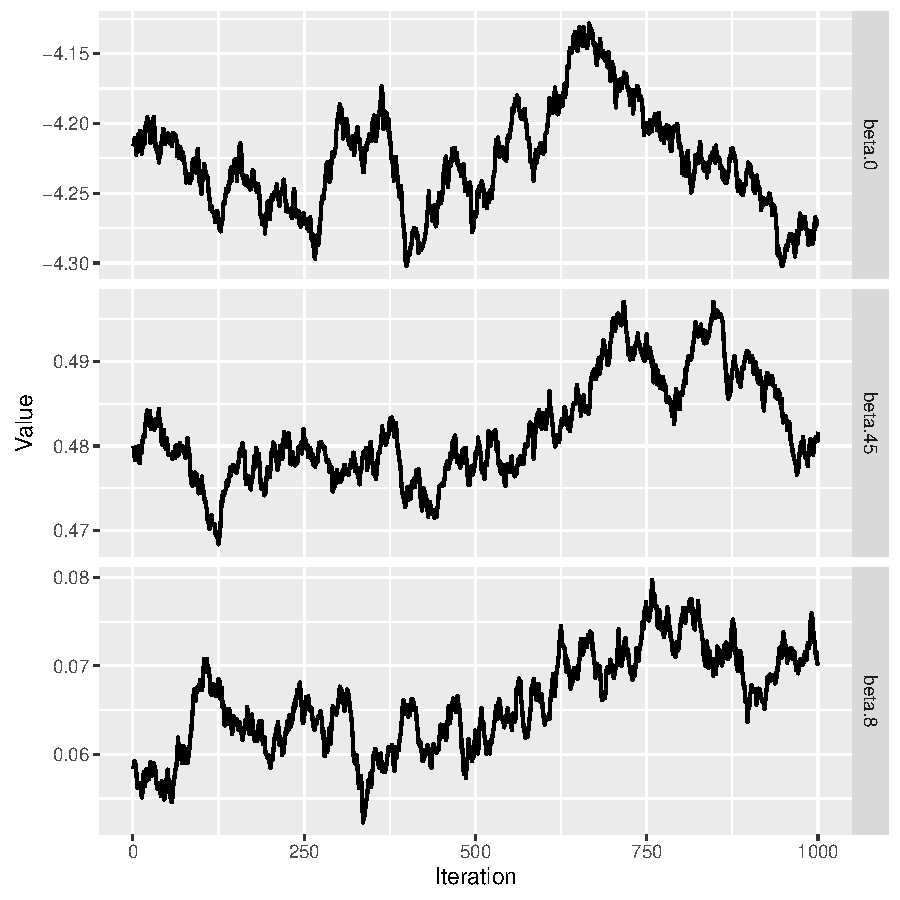
\includegraphics[width=1\textwidth]{traceplot_poisson_da.pdf}
 \caption{Trace plots of three parameters from DA.}
  \label{traceplot_poi_da}
 \end{subfigure}
  \hfill 
 \begin{subfigure}[b]{0.45\textwidth}
 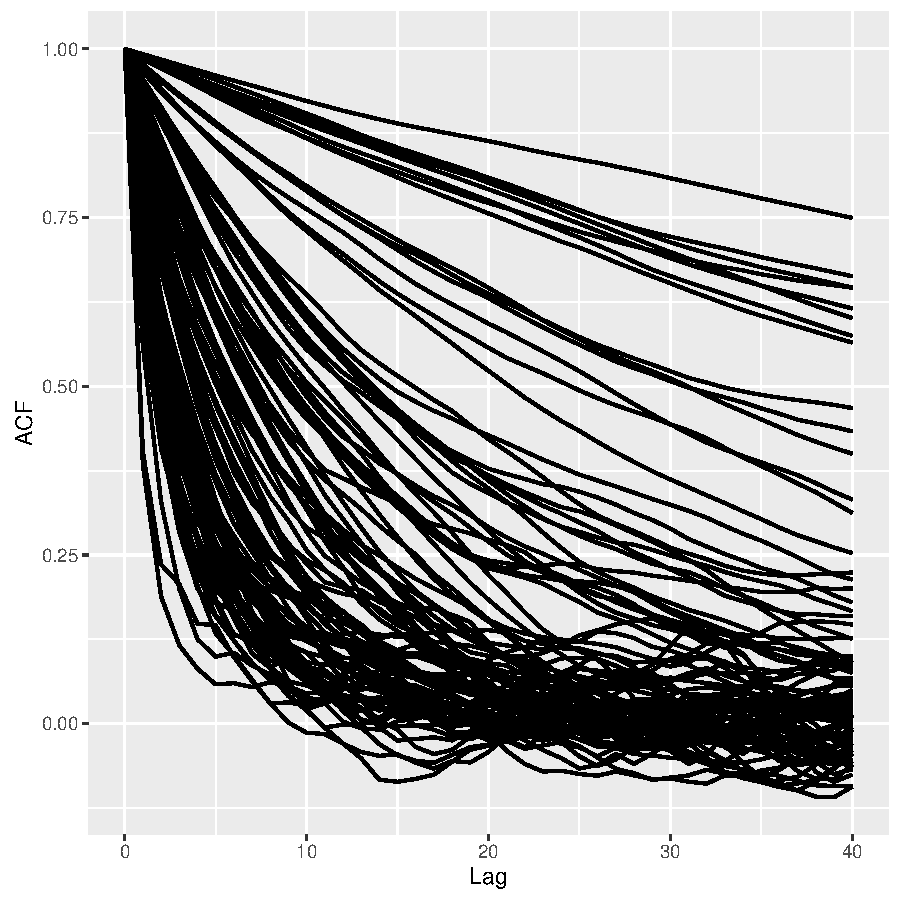
\includegraphics[width=1\textwidth]{poisson_da_acf.pdf}
 \caption{Autocorrelation of all the 96 $\beta$'s from DA.}
   \label{acf_poi_da}
 \end{subfigure} 
  \begin{subfigure}[b]{0.45\textwidth}
 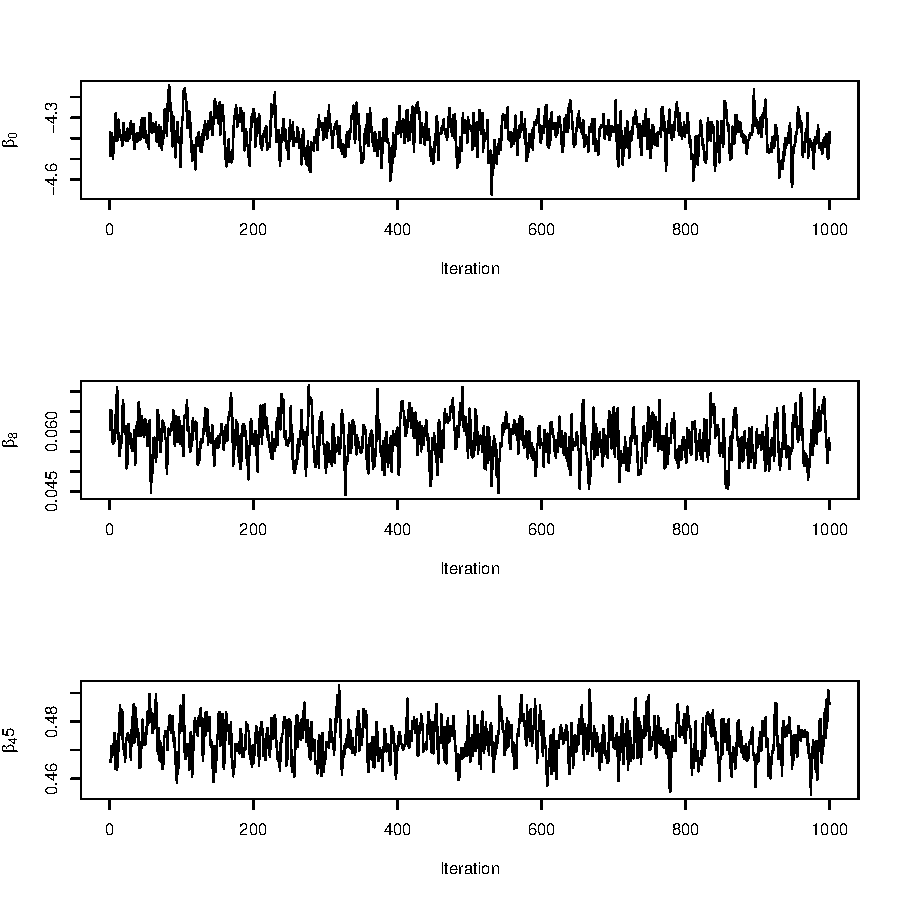
\includegraphics[width=1\textwidth]{traceplot_poisson_ada.pdf}
 \caption{Trace plots of three parameters from CDA.}
  \label{traceplot_poi_ada}
 \end{subfigure}
  \hfill 
 \begin{subfigure}[b]{0.45\textwidth}
 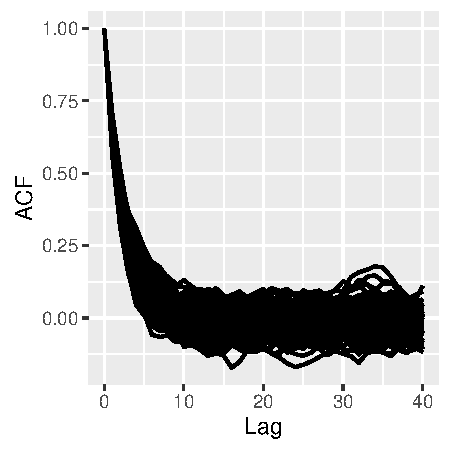
\includegraphics[width=1\textwidth]{poisson_ada_acf.pdf}
 \caption{Autocorrelation of all the 96 $\beta$'s from CDA.}
   \label{acf_poi_ada}
 \end{subfigure}
 \caption{Compared with DA, CDA produces much faster mixing posterior sample.}
 \label{data_poisson}
 \end{figure}



We list the parameter estimates and fit statistics in Table~\ref{table:Poisson}. For simplicity, we include the posterior mean and standard deviation for the intercept $\beta_0$ and the sum of slopes $\sum_{j=1}^{95} \beta_j$. To assess goodness-of-fit, we also evaluate root-mean-squared error $RMSE= \sqrt{ \sum_{i=1}^n  (y_i-\mu_i)^2/n}$ and the deviance $D=2\sum_{i=1}^n \{ y_i \log(y_i/\mu_i) -(y_i-\mu_i)\}$, with $\mu_i=\exp( x_i{\hat\beta})$ and ${\hat\beta}$ the posterior mean. For prediction performance, we use the testing dataset collected $\{ y_{new},  x_{new}\}$ on the same websites and $\tilde y_{i,new}=\exp( x_{i,new}{\hat\beta})$ as the estimator. We evaluate the cross-validation RMSE between $y_{i,new}$ and $\tilde y_{i,new}$.

As expected, the estimate for $\beta_0$ is quite negative, which is captured by the point estimates of both DA and CDA. However, DA severely underestimates the variance of the intercept. The estimates for the $95$ covariates also differ greatly from CDA. Obviously, the poor mixing causes the Markov chain in DA to be trapped in a suboptimal state, whereas CDA performs exceptionally well in fit statistics and the validation error that is almost $4$ times lower. More details in comparing the fitted and prediction are provided in the appendix.

To verify the result, we additionally ran Hamiltonian Monte Carlo (HMC) as the reference. HMC is known for its good mixing properties but very costly evaluation. The result of CDA agrees very well with HMC in both the posterior mean and standard deviation on all the $95$ slope parameters (see appendix for comparison plots). For HMC, it requires significant tuning to reach ideal step size and length for proposal; while CDA only require one additional  step in generating the latent variable. Therefore, CDA is significantly more efficient than HMC and took only $1/10$ of the computing time.


\begin{table}[H]
\centering
\begin{tabular}{|l |r |r| r| r |} 
 \hline
                          & DA & CDA & HMC\\
 [0.5ex]
 \hline
$\beta_0$                         & -4.21 (0.042)& -4.38 (0.075) & -4.47 (0.071) \\
$\sum_{j=1}^{95} \beta_j$         & -0.11 (0.063)& 0.69 (0.053)  & 0.70 (0.055)  \\
RMSE                              & 32.86        & 5.06          & 4.88\\
D                                 & 182127.7     & 107076.9      & 106791.3\\
CV-RMSE                           & 32.01        & 8.61          & 8.28\\
Steps to Converge                 & 2000         & 50            & 500 \\
Computing Time (per 2,000 steps)  & 50 mins       & 51 mins        & 600 mins\\
 \hline
\end{tabular}
\caption{Performance of DA, CDA and HMC in Poisson log-linear regression with online advertisement tracking data. Posterior estimates for the intercept and sum-of-slopes are shown. The CDA shows much better fit statistics such as root-mean-squared error (RMSE) and deviance (D). In cross-validation (CV-RMSE), the CDA outperforms DA as well. The CDA converges much more rapidly than DA. Compared to the reference, CDA agrees with the HMC very well but takes significantly less time.}
\label{table:Poisson}
\end{table}


\section{Discussion}

The slow mixing is a severe problem that prevents data augmentation based MCMC from be applicable on large dataset. With data size increases and become complex, it is common for the parameters to deviate from the area that has reasonable mixing performance. As we show in the previous example, it does not only lead to an un-manageable increase in the computational time, but also could cause Markov chain to be trapped in the suboptimal state.  Therefore, it is necessary to address this issue if we want to keep data augmentation useful in large data.

In this article, we propose a general class of solutions that calibrates this issue. Based on the data augmentation factorization, CDA either integrates out the parameter or increases its conditional variance, so that the step size is adjusted onto the same order of the marginal variance. 

In the data application, we use Hamiltonian Monte Carlo as a good reference for parameter estimation. Here we draw a comparison between the variance increased CDA and HMC.  The ideal Markov chain kernel would be to propose, based on the current state, a state that is as uncorrelated as possible; in the meantime, with high acceptance probability to move to the new state. The HMC utilizes numerical simulation of Hamiltonian dynamics and a long walk to generate such a proposal. In contrast, the CDA directly utilizes the original density but with an increased conditional variance to reduce the correlation. The  short distance between the proposal and current likelihood  enables a good acceptance rate as well. The difference between the two is that the HMC is computationally costly since it relies on evaluation of gradients and multiple Hamiltonian steps for each proposal; whereas CDA does not use gradient but only one-step update, which is almost at the same low cost as the conventional DA method. 


\bibliography{reference}
\bibliographystyle{plainnat}


\section{Appendix}

\subsection{Proof of Theorems}

\subsubsection{Proof of Theorem 1:}


Let $\theta=\{\theta_1, \theta_2\}$ be the parameters that are divided into two parts. Let $\theta'$ and $z'$ be the parameters and latent variables in the last iteration. Omitting $y$ for the ease of notation, the square of maximal correlation can be represented as $||{\bf F}||^2=\underset{s(\theta,z),t(\theta,z)\in L^2(\pi)}{\sup}\;\mbox{corr}\{s(\theta,z),t(\theta^{'},z')\}^2
= \underset{s(\theta,z)\in L^2(\pi)}{\sup}\; \frac{\mbox{var} [ E \{ s(\theta,z)|\theta^{'},z'\}]}{\mbox{var}\{s(\theta,z) \} }$.

The original DA samples in the order of $ \{\theta'_1, \theta'_2\} \rightarrow z' \rightarrow \{\theta_1, \theta_2\}\rightarrow z$, with $ \mbox{var} [ E \{ s(\theta,z)|\theta^{'},z'\}] =  \mbox{var} [ E \{ s(\theta_1, \theta_2,z)|\theta^{'}_1,\theta^{'}_2,z'\}] $. The marginalization and sampling based CDA samples  in the order of $ \theta'_2 \rightarrow z' \rightarrow \theta_2\rightarrow z$, followed by $z' \rightarrow \theta'_1$ and  $z \rightarrow \theta_1$ with $ \mbox{var} [ E \{ s(\theta,z)|\theta^{'},z'\}] =  \mbox{var} [ E \{ s(\theta_1, \theta_2,z)|\theta^{'}_1,\theta^{'}_2,z'\}] = \mbox{var} [ E \{ s(\theta_1, \theta_2,z)|\theta^{'}_2,z'\}]$.

For better clarity, let $E_{X}$ denote the integration over $P(dX)$. 

\begin{equation}
\begin{aligned}
 \mbox{var} [ E \{ s(\theta_1, \theta_2,z)|\theta^{'}_2,z'\}]  & = E_{\theta^{'}_2,z'}  [ E_{\theta_1, \theta_2,z}\{ s(\theta_1, \theta_2,z)|\theta^{'}_2,z' \} ]^2 -  (E_{\theta^{'}_2,z'}   [ E_{\theta_1, \theta_2,z}\{ s(\theta_1, \theta_2,z)|\theta^{'}_2,z' \} ])^2  \\
 & = E_{\theta^{'}_2,z'}   [ E_{\theta'_1}E_{\theta_1, \theta_2,z} \{ s(\theta_1, \theta_2,z)|\theta'_1, \theta^{'}_2,z' \} ]^2 - (E_{\theta^{'}_1,\theta^{'}_2,z'}   [ E_{\theta_1, \theta_2,z} \{ s(\theta_1, \theta_2,z)|\theta^{'}_1,\theta^{'}_2,z' \} ])^2 \\
& \le  E_{\theta^{'}_2,z'}  E_{\theta'_1} [ E_{\theta_1, \theta_2,z} \{ s(\theta_1, \theta_2,z)|\theta'_1, \theta^{'}_2,z' \} ]^2 - (E_{\theta^{'}_1,\theta^{'}_2,z'}   [ E_{\theta_1, \theta_2,z} \{ s(\theta_1, \theta_2,z)|\theta^{'}_1,\theta^{'}_2,z' \} ])^2\\
& =  \mbox{var}  [E \{ s(\theta_1, \theta_2,z)|\theta^{'}_1,\theta^{'}_2,z'\}] 
\end{aligned}
\end{equation}

This completes the proof.


\subsubsection{Proof of Theorem 2:}

Both DA and the variance increase CDA sample in the order of  $\theta' \rightarrow z' \rightarrow \theta \rightarrow z$. Omitting $y$ for the ease of notation, by Lemma 4 of \cite{liu1994collapsed}, $\underset{s(\theta)\in L^2(\pi)}{\sup}\; \frac{\mbox{var} [ E \{ s(\theta,z)|\theta^{'},z'\}]}{\mbox{var}\{s(\theta,z) \} } = \underset{s(\theta)\in L^2(\pi)}{\sup}\; \frac{\mbox{var} [ E \{ s(\theta)|z'\}]}{\mbox{var}\{s(\theta) \} }$.

As  $\frac{ var_{IV}\{ \theta|z\}}{ var\{ \theta | z\}} \ge (1+\epsilon) $ leads to  $E    [var_{IV}\{ \theta|z\}] \ge (1+\epsilon) E[var\{ \theta|z\}]$, $\frac{|\mbox{var}\{s(\theta)  \} - \mbox{var}_{IV}\{s(\theta)\}| }{\mbox{var}\{s(\theta) \} }\le \epsilon$ leads to $ \mbox{var}_{IV}\{s(\theta)  \} \le (1+\epsilon)  \mbox{var}\{s(\theta) \} $.

\begin{equation}
\begin{aligned}
1- \frac{E    [var_{IV}\{ \theta|z\}]}{\mbox{var}_{IV}\{s(\theta) \}} \le 1- \frac{ (1+\epsilon) E[var\{ \theta|z\}]}{(1+\epsilon)  \mbox{var}\{s(\theta) \} }
\end{aligned}
\end{equation}

Using $\mbox{var} \{ s(\theta)\} = E    [var\{ s(\theta)|z\}] + var    [E\{ s(\theta)|z\}]$ and taking supremum on both sides complete the proof.


\subsubsection{Proof of Theorem 3:}

Without loss of generality, take $M\ge 1$, then $E |\theta_j| {1}_{|\theta_j|>M}\le E \theta_j^2 {1}_{|\theta_j|>M}\le \epsilon_2$.

\begin{equation}
\begin{aligned}
|E (\theta_j |y)-E_{r,b} (\theta_j |y)| & = \int  | \theta_j \pi(\theta_j | y) -  \theta_j\pi_{r,b}(\theta_j|y)| d\theta_j  \\
& \le \int  | \theta_j| |\pi(\theta_j | y) - \pi_{r,b}(\theta_j|y)| d\theta_j  \\
& =   \int  1(|\theta_j|\le M) | \theta_j|\cdot |\pi(\theta_j | y) - \pi_{r,b}(\theta_j|y)| d\theta_j  +  \int 1(|\theta_j|>M) | \theta_j| |\pi(\theta_j | y) - \pi_{r,b}(\theta_j|y)| d\theta_j  \\
& \le M   \int   |\pi(\theta_j | y) - \pi_{r,b}(\theta_j|y)| d\theta_j  + \int 1(|\theta_j|>M) | \theta_j| \pi(\theta_j | y) d\theta_j +  \int 1(|\theta_j|>M) | \theta_j| \pi_{r,b}(\theta_j|y) d\theta_j  \\
& \le 2M\epsilon_1 + 2\epsilon_2 \\
& = 2M\epsilon_1 + o(\epsilon_1),
\end{aligned}
\end{equation}
where triangle inequality and the definition of total variation distance are used.



\begin{equation}
\begin{aligned}
|\mbox{var} (\theta_j |y)-\mbox{var}_{r,b} (\theta_j |y)| & = | [E (\theta^2_j |y)- \{ E(\theta_j |y)\}^2] - [ E_{r,b} (\theta^2_j |y)-\{ E_{r,b} (\theta_j |y)\}^2 ]|\\
& \le | E (\theta^2_j |y)-  [ E_{r,b} (\theta^2_j |y) ] |+ | \{ E(\theta_j |y)\}^2 -\{ E_{r,b} (\theta_j |y)\}^2 ]|\\
& \le 2M^2 \epsilon_1 + 2\epsilon_2 + | \{ E(\theta_j |y)\} -\{ E_{r,b} (\theta_j |y)\} ]| \cdot | \{ E(\theta_j |y)\}+\{ E_{r,b} (\theta_j |y)\}]| \\
& \le 2M^2 \epsilon_1 + 2\epsilon_2 +  (2M\epsilon_1 + 2\epsilon_2) \{  2 E(\theta_j |y) + 2M\epsilon_1 + 2\epsilon_2 \} \\
& \le 2M^2 \epsilon_1 + 2\epsilon_2 +  (2M\epsilon_1 + 2\epsilon_2) \{  2 M+ 2\epsilon_2 + 2M\epsilon_1 + 2\epsilon_2 \} \\
& = 6M^2\epsilon_1 + o(\epsilon_1).
\end{aligned}
\end{equation}


To prove Corollary 1, using Cauchy-Schwarz inequality $ \{  E\theta_{j_1}\theta_{j_2} 1(\theta_{j_1}>M_{j_1} )  1(\theta_{j_2}>M_{j_2} )    \}^2 \le   E\theta^2_{j_1}1(\theta_{j_1}>M_{j_1} )  E \theta^2_{j_2} 1(\theta_{j_1}>M_{j_2} )   =\epsilon^2_2$. Following the similar proof for variance, it can be derived that:

$$|\mbox{cov}(\theta_{j_1},\theta_{j_2}|y)-\mbox{cov}_{r,b}(\theta_{j_1},\theta_{j_2}|y)|\le 6M_{j_1}M_{j_2}\epsilon_1+o(\epsilon_1 ).$$

\subsubsection{Proof of Theorem 4:}

Since $\theta= B^{-} B\theta$, $\mbox{cov} B\theta= B^{-}  \mbox{cov} B\theta B^{-T} $, applying H\"older's inequality:

$$||{E}\theta-{E}\theta_{r,b}||_1 \le ||B^{-}||_1 ||{E}B\theta- {E}B\theta_{r,b}||_\infty$$
$$||\mbox{cov}\theta-\mbox{cov}\theta_{r,b}||_1 \le  ||B^{-}||_\infty ||B^{-}\mbox{cov} B\theta- B^{-}\mbox{cov}B\theta_{r,b}||_1 \le ||B^{-}||_1 ||B^{-}||_\infty ||\mbox{cov} B\theta- \mbox{cov}B\theta_{r,b}||_\infty$$

\subsection{Approximation Error in Logistic Regression}

For better clarity, we renumber the double index $ij$ using single index $i$.

\subsubsection{Total Variation Distance}

The individual Kullback-Leibler distance:

\begin{equation}
\begin{aligned}
KL\{ { L_{r,b}(y_i|\eta_{i}) } || {L(y_i|\eta_{i})} \}& =\mbox{E}\log \frac{\Gamma(1/r_i+1) r_i^{y_i}  /\Gamma(1/r_i -y_i+1)  }{\Gamma(2) /\Gamma(2 -y_i)  } + \log \frac{ 1+\exp(\eta_{i})}{ \{1+\exp(\eta_{i})r_i\}^{1/r_i}}\\
& =\log\{1+ \exp ( \eta_{i})\}   - 1/r \log\{1+ r\exp ( \eta_{i})\}\\
& \le   \{   (r_i-1) \frac{ \exp(2\eta_{i})}{2} \}  1\{\exp(\eta_{i})< 1/r_i\} + \log \frac{ 1+\exp(\eta_{i})}{ \{1+\exp(\eta_{i})r_i\}^{1/r_i}}  1\{\exp(\eta_{i})\ge 1/r_i\} \\
%& \le   \frac{r_i-1}{2 r_i^2}  1\{r_i <\exp(-\eta_{i}) \} + \log \frac{ 1+\exp(\eta_{i})}{ \{1+\exp(\eta_{i})r_i\}^{1/r_i}}  1\{ \eta_{i} \ge -\log r_i\}.
\label{KL_logit}
\end{aligned}
\end{equation}


With adaptive $r_i=1$ if $\eta_{i}\ge -\log r_i$ and Pinsker's inequality,

$$||P_{r,b}(y_i|\eta_{i}) - P(y_i|\eta_{i})||_{TV} \le   \{   \frac{\sqrt{r_{i}-1}  \exp(\eta_{i})}{2} \} 1 \{\eta_{i}< - \log r_{i} \le 0 \}$$

\subsubsection{Tail Integral}

Consider each likelihood $L(y_i|p_i) = p^y_i (1-p)^{1-y_i}$ with $p_i=\frac{\exp(\eta_{i})}{1+\exp(\eta_{i})}$. Applying density transformation leads to 
$\pi(\eta_{i}|y_i) = \frac{\exp(\eta_{i}) \exp(y_i\eta_{i})}{\{1+\exp(\eta_{i})\}^3}$.

If $y_i=1$,
\begin{equation}
	\begin{aligned}
			\mbox{E}\{ \eta_{i}^2 1(|\eta_{i}|>M) \} & = E\{ \eta_{i}^2 1(|\eta_{i}|>M, \eta_{i} \ge 0 ) \} + E\{ \eta_{i}^2 1(|\eta_{i}|>M, \eta_{i}<0 ) \} \\
	& \le \int_M^{\infty} \frac{\eta_{i}^2}{1+\exp(\eta_{i})} d\eta_{i} + \int_{-\infty}^{-M}{\eta_{i}^2}{\exp(2\eta_{i})}d\eta_{i}  \\
	& \le \int_M^{\infty} {\eta_{i}^2}{\exp(-\eta_{i})} d\eta_{i} +\int_{-\infty}^{-M}{\eta_{i}^2}{\exp(2\eta_{i})}d\eta_{i} \\
	& = (M^2+2M+2)\exp(-M) + \frac{1}{4} (2M^2 + 2M +1) \exp(-2M).
	\end{aligned}
\end{equation}

if $y_i=0$,
\begin{equation}
	\begin{aligned}
			\mbox{E}\{ \eta_{i}^2 1(|\eta_{i}|>M) \} & = \mbox{E}\{ \eta_{i}^2 1(|\eta_{i}|>M, \eta_{i} \ge 0 ) \} + E\{ \eta_{i}^2 1(|\eta_{i}|>M, \eta_{i}<0 ) \} \\
	& \le \int_M^{\infty} \frac{\eta_{i}^2}{\{1+\exp(\eta_{i})\}^2} d\eta_{i} + \int_{-\infty}^{-M}{\eta_{i}^2}{\exp(\eta_{i})}d\eta_{i}  \\
	& \le \int_M^{\infty} {\eta_{i}^2}{\exp(-2\eta_{i})} d\eta_{i} + \int_{-\infty}^{-M}{\eta_{i}^2}{\exp(\eta_{i})}d\eta_{i} \\
	& =\frac{1}{4} (2M^2 + 2M +1) \exp(-2M)+  (M^2+2M+2)\exp(-M) .
	\end{aligned}
\end{equation}

Therefore, the tail square integral is in $O(M^2 \exp(-M))$.


Consider the approximate density $L_{r,b} (y_i| \eta_i) =\frac{\Gamma(1/r_i+1)}{\Gamma(1/r_i-y_i+1)\Gamma(y_i+1)} p^{y_i} (1-p)^{(1/r_i-y_i)}$, where $p=\frac{\exp ( \eta_i+\log r_i)}{\{1+ \exp ( \eta_i +\log r_i)\}}$ and $y_i< 1/r_i+1$.  Applying density transformation leads to $\pi(\eta_{i}|y_i) = \frac{\Gamma(1/r_i+1)}{\Gamma(1/r_i-y_i+1)\Gamma(y_i+1)}\frac{\{r_i\exp(\eta_{i})\}^{(y_i+1)}}{\{1+r_i\exp(\eta_{i})\}^{(1/r_i+2)}}$.

\begin{equation}
	\begin{aligned}
			\mbox{E}_{r,b}\{ \eta_{i}^2 1(|\eta_{i}|>M) \}  % = \mbox{E}_{r,b}\{ \eta_{i}^2 1(|\eta_{i}|>M, \eta_{i} \ge 0 ) \} + \mbox{E}_{r,b}\{ \eta_{i}^2 1(|\eta_{i}|>M, \eta_{i}<0 ) \} \\
	&	 \le      \int      \eta_i^2  1(|\eta_{i}|>M)  \frac{\Gamma(1/r_i+1)r_i^{y_i}}{\Gamma(1/r_i-y_i+1)}\frac{r_i}{\Gamma(y_i+1)}\frac{\{\exp(\eta_{i})\}^{(y_i+1)}}{\{1+r_i\exp(\eta_{i})\}^{(1/r_i+2)}} d\eta_i  \\
	&  \le \int \eta_i^2  1(|\eta_{i}|>M) \frac{r_i}{y_i!}\frac{\{\exp(\eta_{i})\}^{(y_i+1)}}{\{1+r_i\exp(\eta_{i})\}^{(1/r_i+2)}} d\eta_i  \\	
		& \le \frac{1}{y_i! r_i^{y_i}} \int_M^{\infty} \frac{\eta_{i}^2}{1+r_i\exp(\eta_{i})} d\eta_{i} +  \frac{r_i}{y_i!} \int_{-\infty}^{-M}{\eta_{i}^2}{\exp\{\eta_{i} (y_i+1) \}}d\eta_{i} \\
		& \le \frac{1}{y_i! r_i^{y_i+1}} \int_M^{\infty} {\eta_{i}^2}{\exp(-\eta_{i})} d\eta_{i} +  \frac{r_i}{y_i!} \int_{-\infty}^{-M}{\eta_{i}^2}{\exp\{\eta_{i} (y_i+1) \}}d\eta_{i} \\
	& = \frac{1}{y_i! r_i^{y_i+1}} (M^2+2M+2)\exp(-M) + \frac{r_i}{y_i!}   (M^2+2M+2)\exp(-M) 
	\end{aligned}
\end{equation}

\subsection{Approximation Error in Poisson Log-Linear Model}

\subsubsection{Total Variation Distance}

With $\eta_i=\xbeta$, the individual Kullback-Leibler distance:

\begin{equation}
\begin{aligned}
KL\{ { L_{r,b}(y_i|\eta_{i}) } || {L(y_i|\eta_{i})} \}& =\mbox{E}\log \frac{\Gamma(1/r_i+1) r_i^{y_i}  }{\Gamma(1/r_i -y_i+1)   } + \log \frac{ \exp\exp(\eta_{i})}{ \{1+\exp(\eta_{i})r_i\}^{1/r_i}}\\
& \le \exp ( \eta_{i})   - 1/r \log\{1+ r\exp ( \eta_{i})\}\\
& \le   \{   r_i \frac{ \exp(2\eta_{i})}{2} \}  1\{\exp(\eta_{i})< 1/r_i\} + \log \frac{ \exp\exp(\eta_{i})}{ \{1+\exp(\eta_{i})r_i\}^{1/r_i}} 1\{\exp(\eta_{i})\ge 1/r_i\} \\
\label{KL_poisson}
\end{aligned}
\end{equation}

With adaptive $r_i = 0$ if $\eta_{i}\ge 1/r_i$ and Pinsker's inequality,
$$||P_{r,b}(y_i|\eta_{i}) - P(y_i|\eta_{i})||_{TV} \le   \{   \frac{\sqrt{r_{i}}  \exp(\eta_{i})}{2} \} 1 \{\eta_{i}< - \log r_{i} \}$$



\subsubsection{Tail Integral}


Consider each likelihood $L(y_i|p_i) = {p_i^{y_i}\exp(-p_i)}/{y_i!}$ with $p_i={\exp(\eta_{i})}$. Applying density transformation leads to 
$\pi(\eta_{i}|y_i) = \exp \{\eta_i (y_i+1)\} \exp\{-\exp(\eta_i) \} /{y_i!}$. Without loss of generality, assume $|M|\ge 1$.


\begin{equation}
	\begin{aligned}
			E\{ \eta_{i}^2 1(|\eta_{i}|>M) \} & = E\{ \eta_{i}^2 1(|\eta_{i}|>M, \eta_{i} \ge 0 ) \} + E\{ \eta_{i}^2 1(|\eta_{i}|>M, \eta_{i}<0 ) \} \\
	& \le \int_M^{\infty}  \frac{ \exp \{\eta_i (y_i+3)\}  \} }{\exp\{\exp(\eta_i)\} e^2 y_i!} d\eta_{i} + \int_{-\infty}^{-M}  \frac {\eta_{i}^2 \exp \{ \eta_{i} (y_i+1)\}  }{ y_i !}d\eta_{i}  \\
	& =  \frac{IGamma(y_i+3, \exp(M)\} }{e^2 y_i!} +   \frac{IGamma(3, (y_i+1)M)\} }{(y_i+1)^3 y_i!} .
	\end{aligned}
\end{equation}
where $IGamma(a,b)$ is the incomplete Gamma function $\int_b^{\infty} t^{a-1} \exp(-t) dt$, equal to the $\{1-F(b) \} \Gamma(a)$, with $F(b)$ as the cumulative distribution function of gamma distribution ${\mathcal G}(a,1)$.


Similar to the logistic approximate, consider the approximate density $L_{r,b} (y_i| \eta_i) =\frac{\Gamma(1/r_i+1)}{\Gamma(1/r_i-y_i+1)\Gamma(y_i+1)} p^{y_i} (1-p)^{(1/r_i-y_i)}$, where $p=\frac{\exp ( \eta_i+\log r_i)}{\{1+ \exp ( \eta_i +\log r_i)\}}$ and $y_i< 1/r_i+1$.  Applying density transformation leads to $\pi(\eta_{i}|y_i) = \frac{\Gamma(1/r_i+1)}{\Gamma(1/r_i-y_i+1)\Gamma(y_i+1)}\frac{\{r_i\exp(\eta_{i})\}^{(y_i+1)}}{\{1+r_i\exp(\eta_{i})\}^{(1/r_i+2)}}$.


Note when $\eta_i>0$ hence $r_i < 1/exp(0)=1$, $\frac{1}{1+r_i\exp(\eta_{i})\}^{(1/r_i)}}\le \frac{1}{1+ \exp(\eta_{i})} $. Then,

\begin{equation}
	\begin{aligned}
			\mbox{E}_{r,b}\{ \eta_{i}^2 1(|\eta_{i}|>M) \}  % = \mbox{E}_{r,b}\{ \eta_{i}^2 1(|\eta_{i}|>M, \eta_{i} \ge 0 ) \} + \mbox{E}_{r,b}\{ \eta_{i}^2 1(|\eta_{i}|>M, \eta_{i}<0 ) \} \\
	&	 \le      \int      \eta_i^2  1(|\eta_{i}|>M)  \frac{\Gamma(1/r_i+1)r_i^{y_i}}{\Gamma(1/r_i-y_i+1)}\frac{r_i}{\Gamma(y_i+1)}\frac{\{\exp(\eta_{i})\}^{(y_i+1)}}{\{1+r_i\exp(\eta_{i})\}^{(1/r_i+2)}} d\eta_i  \\
	&  \le \int \eta_i^2  1(|\eta_{i}|>M) \frac{r_i}{y_i!}\frac{\{\exp(\eta_{i})\}^{(y_i+1)}}{\{1+r_i\exp(\eta_{i})\}^{(1/r_i+2)}} d\eta_i  \\	
		& \le \int_M^{\infty} \frac{r_i}{y_i! r_i^{y_i+1}}\frac{\eta_i^2}{\{1+r_i\exp(\eta_{i})\}} d\eta_i 
				+  \frac{r_i}{y_i!} \int_{-\infty}^{-M}{\eta_{i}^2}{\exp\{\eta_{i} (y_i+1) \}}d\eta_{i} \\
	& =  \frac{1}{y_i! r_i^{(y_i+1)}}   (M^2+2M+2)\exp(-M) + \frac{r_i}{y_i!}    \frac{IGamma(3, (y_i+1)M)\} }{(y_i+1)^3 }
	\end{aligned}
\end{equation}



\subsection{Mixing of Zero-inflated Poisson without Calibration}


 \begin{figure}[H]
 % \centering
   \begin{subfigure}[b]{0.45\textwidth}
 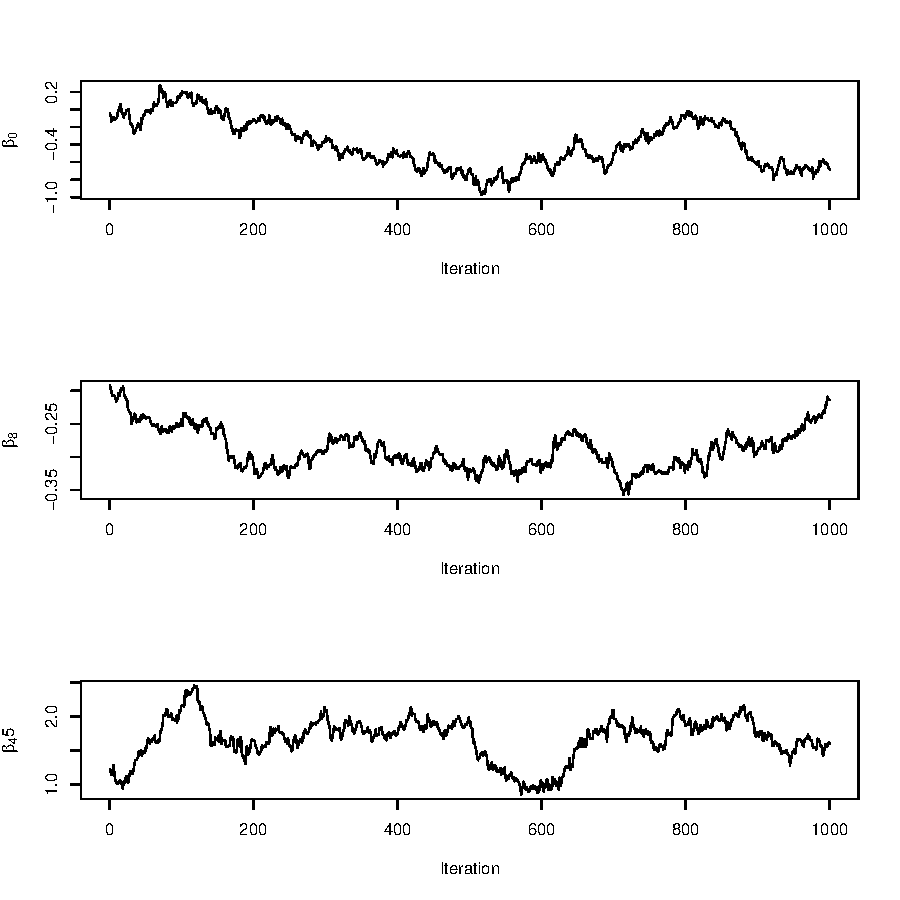
\includegraphics[width=1\textwidth]{traceplot_poisson_zip_da.pdf}
 \caption{Trace plots of three parameters from DA ZIP model}
 \end{subfigure}
  \hfill 
 \begin{subfigure}[b]{0.45\textwidth}
 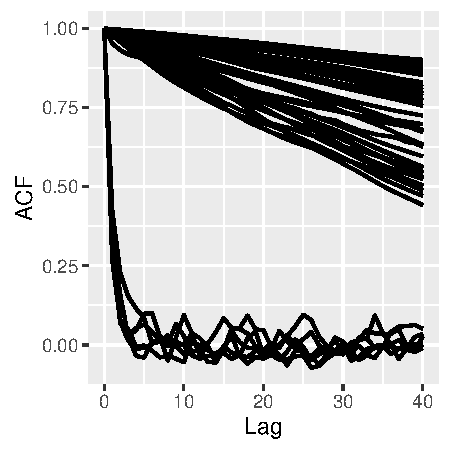
\includegraphics[width=1\textwidth]{poisson_zip_da_acf.pdf}
 \caption{Autocorrelation of all the 96 $\beta$'s from DA ZIP model.}
 \end{subfigure}  
 \caption{The hierarchy in the zero-inflated Poisson model does NOT help reduce the autocorrelation.}
 \end{figure}



\subsection{Goodness-of-Fit and Cross-Validation for Poisson Regression}


 \begin{figure}[H]
 % \centering
   \begin{subfigure}[b]{0.45\textwidth}
 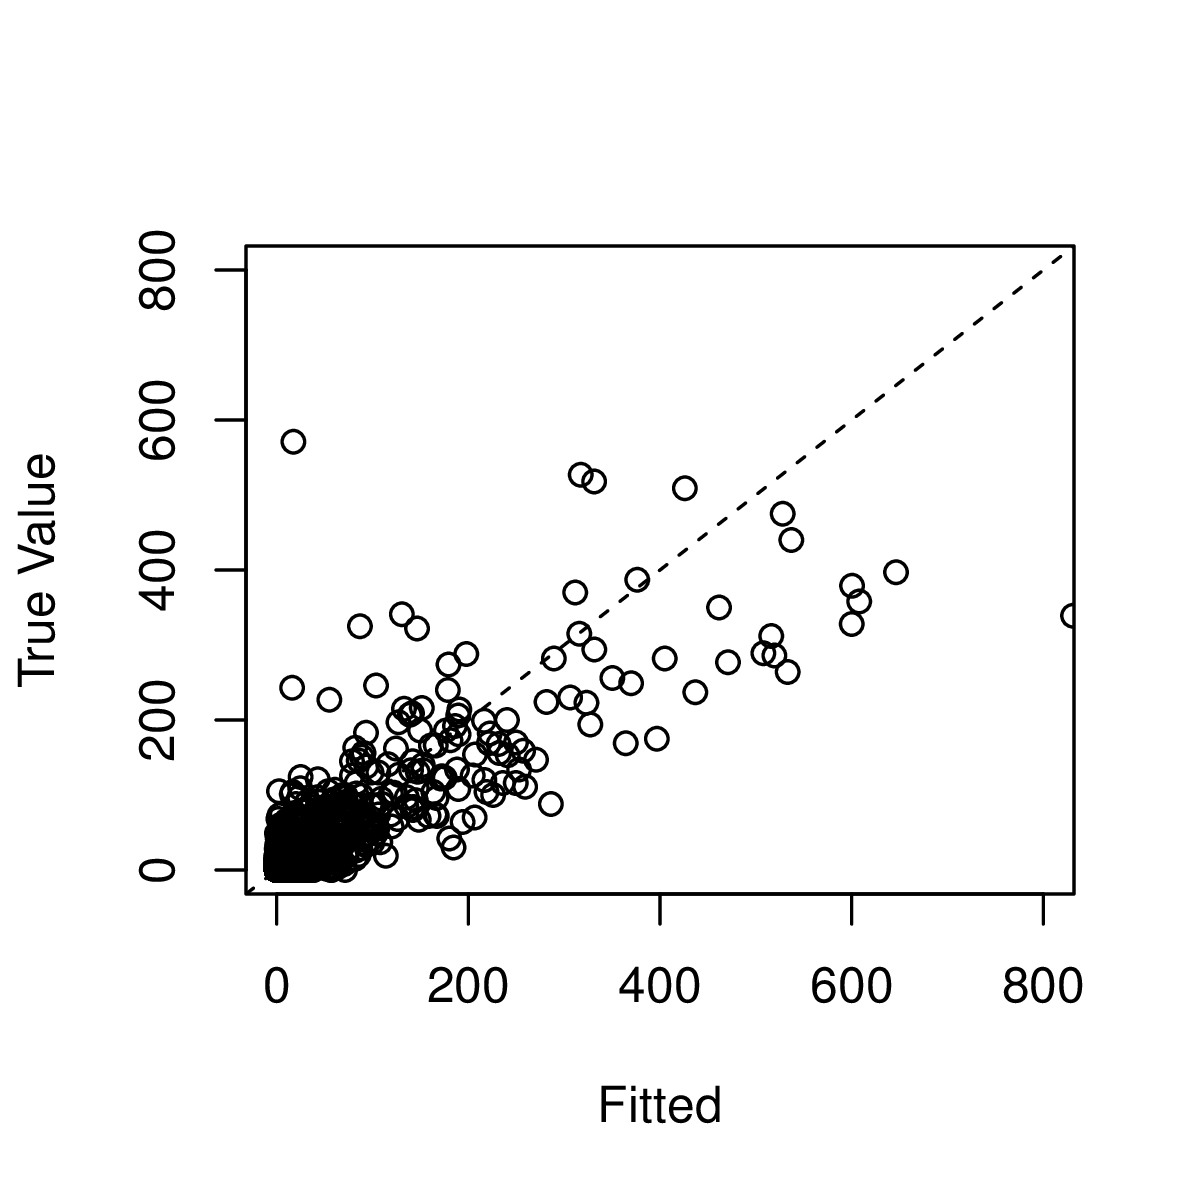
\includegraphics[width=1\textwidth]{poisson_fitting_da.png}
 \caption{Fitted vs true values using DA}
 \end{subfigure}
  \hfill 
 \begin{subfigure}[b]{0.45\textwidth}
 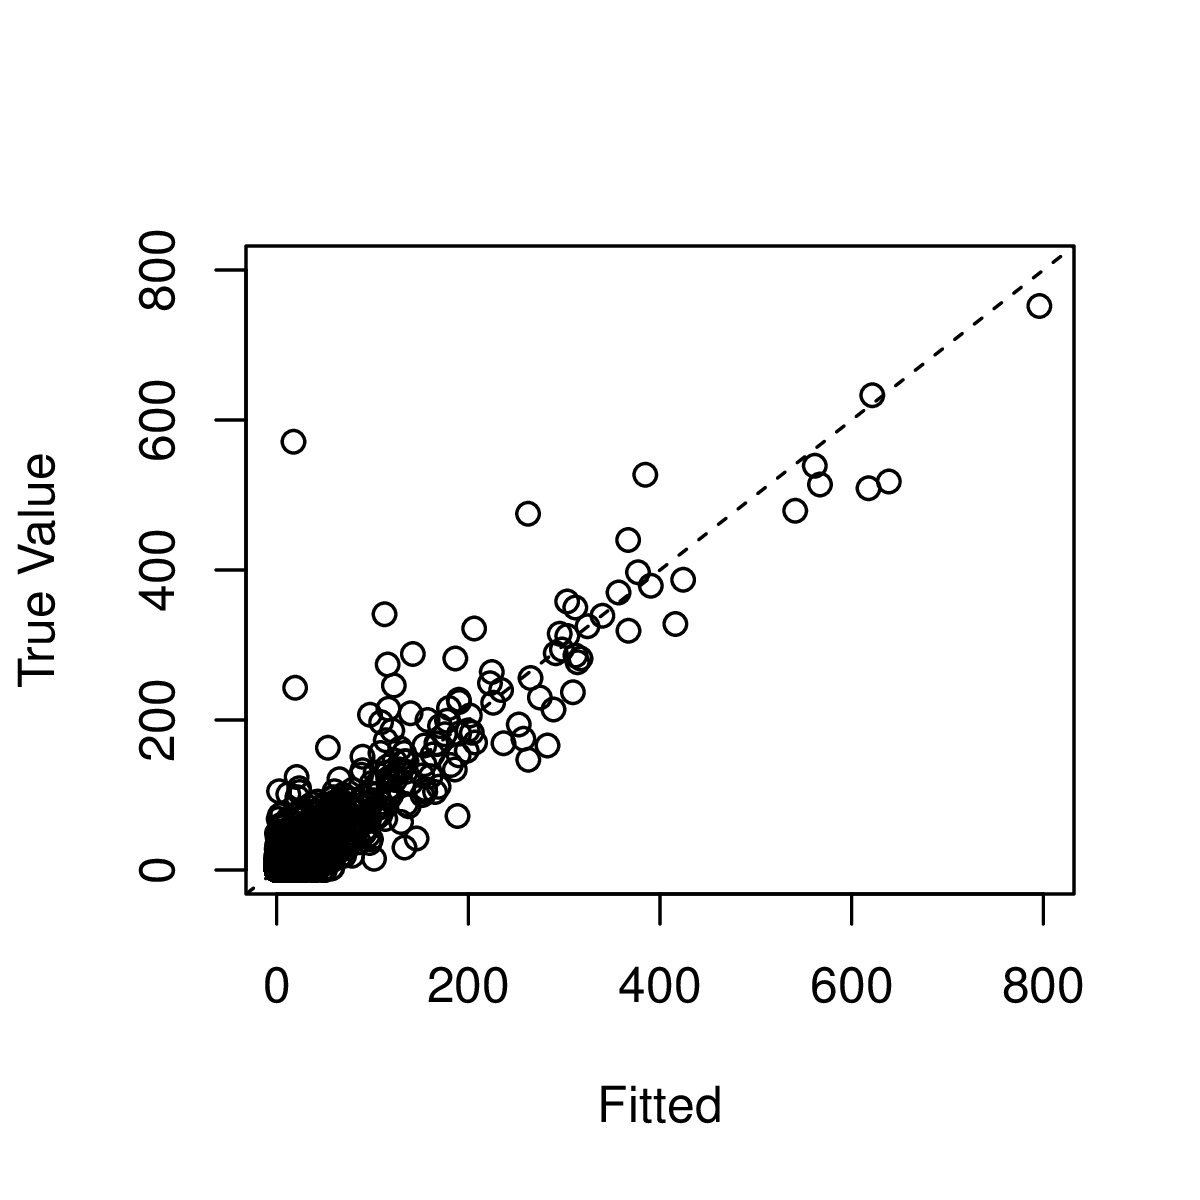
\includegraphics[width=1\textwidth]{poisson_fitting_ada.png}
 \caption{Fitted vs true values using CDA}
 \end{subfigure}  
   \begin{subfigure}[b]{0.45\textwidth}
 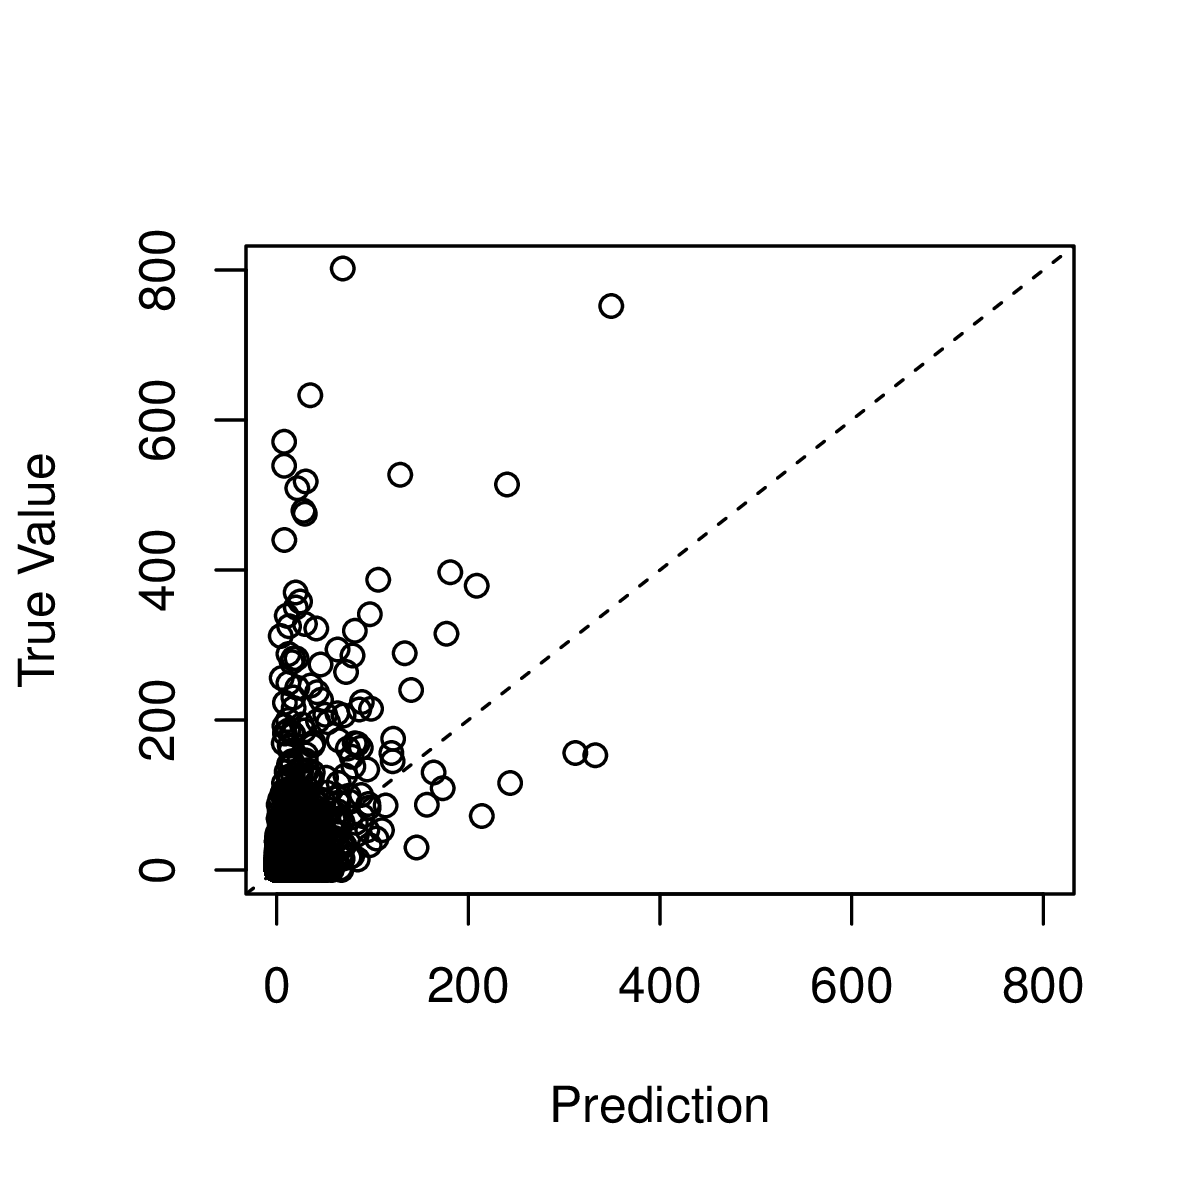
\includegraphics[width=1\textwidth]{poisson_cv_da.png}
 \caption{Prediction vs true values using DA}
 \end{subfigure}
  \hfill 
 \begin{subfigure}[b]{0.45\textwidth}
 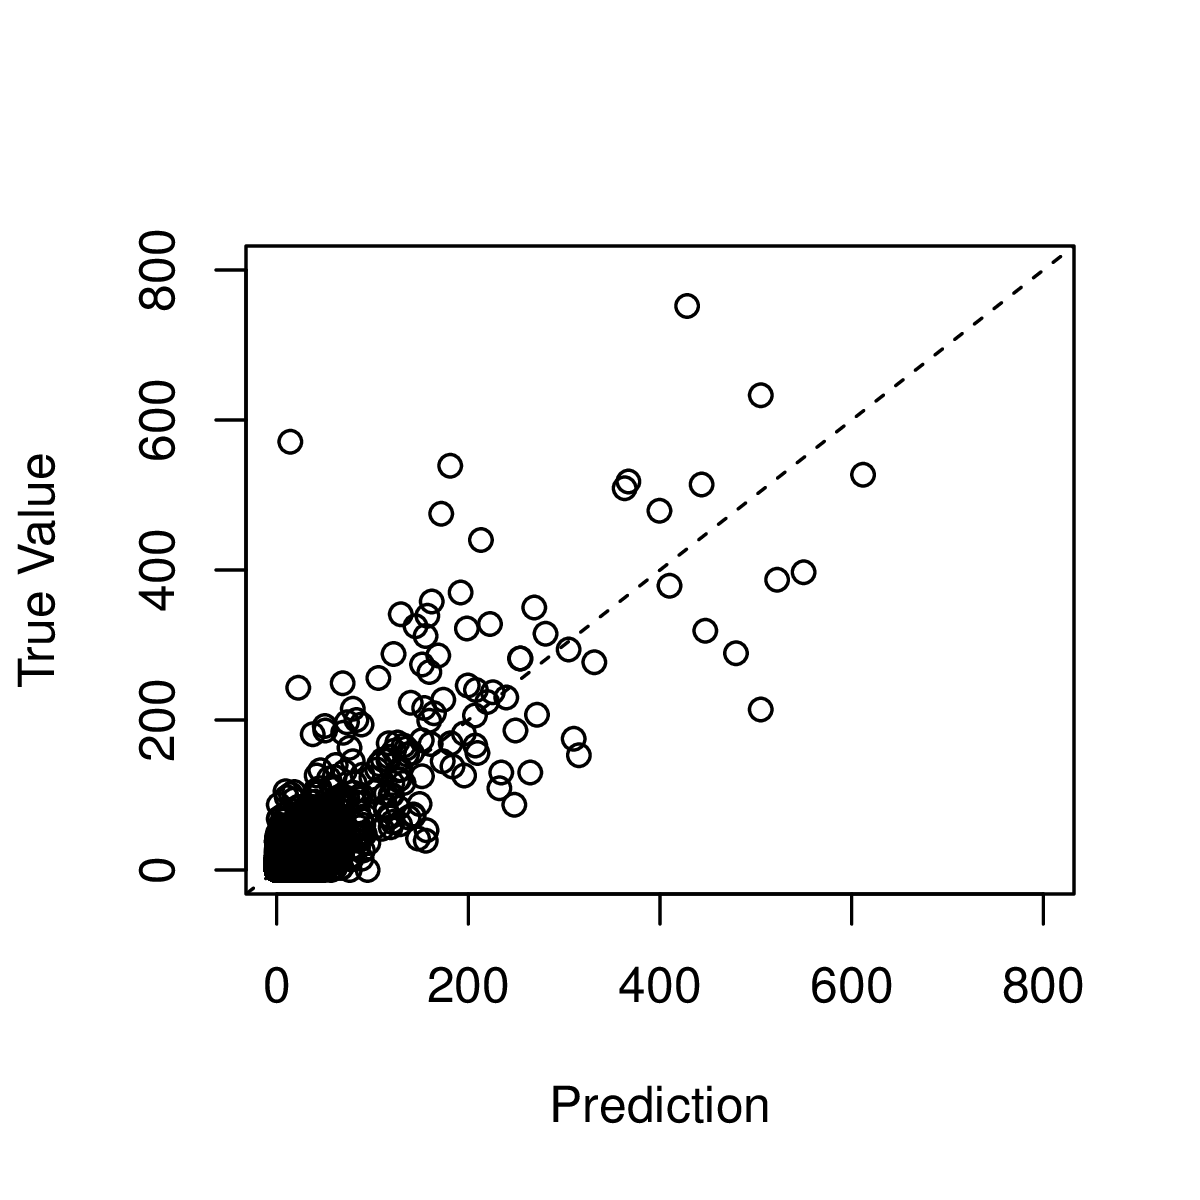
\includegraphics[width=1\textwidth]{poisson_cv_ada.png}
 \caption{Prediction vs true values using CDA}
 \end{subfigure} 
 \caption{The posterior estimates produced by CDA is better fitted to the data and have more accurate prediction than DA.}
 \end{figure}

 \subsection{Comparing posterior samples of CDA with HMC}


\begin{figure}[H]
 % \centering
   \begin{subfigure}[b]{0.45\textwidth}
 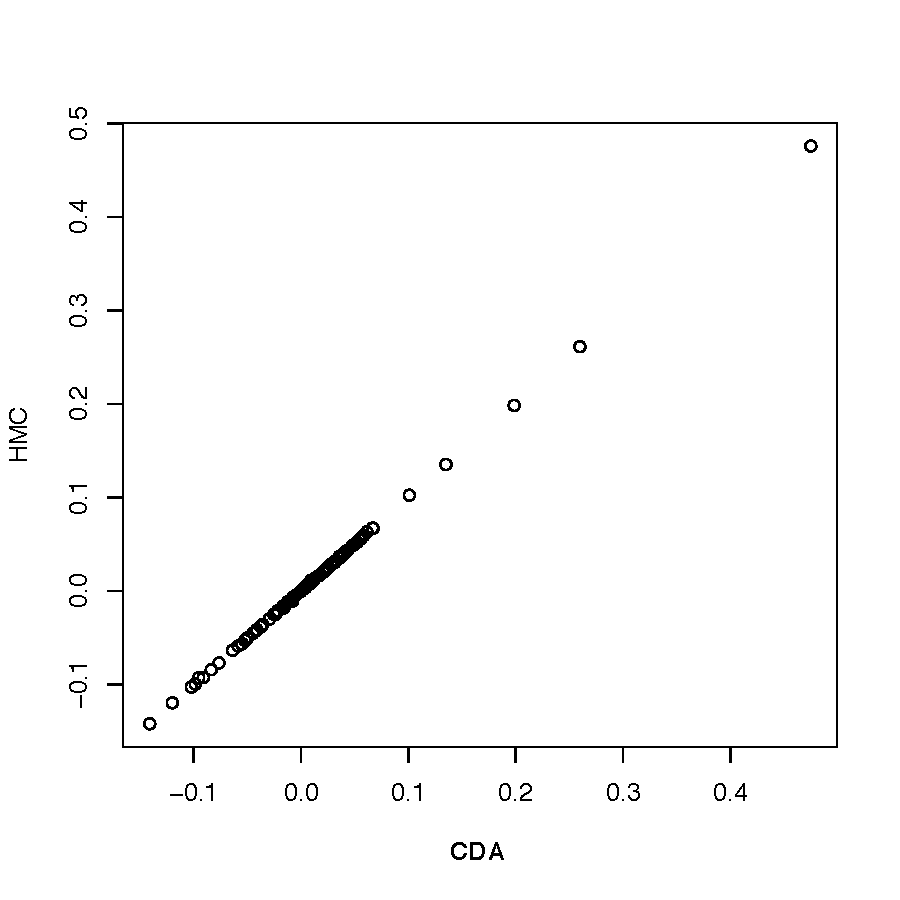
\includegraphics[width=1\textwidth]{CDAvsHMC_mean.pdf}
 \caption{Comparing posterior means for $\beta_1,\dots \beta_{95}$ from the HMC and CDA.}
 \end{subfigure}
  \hfill 
 \begin{subfigure}[b]{0.45\textwidth}
 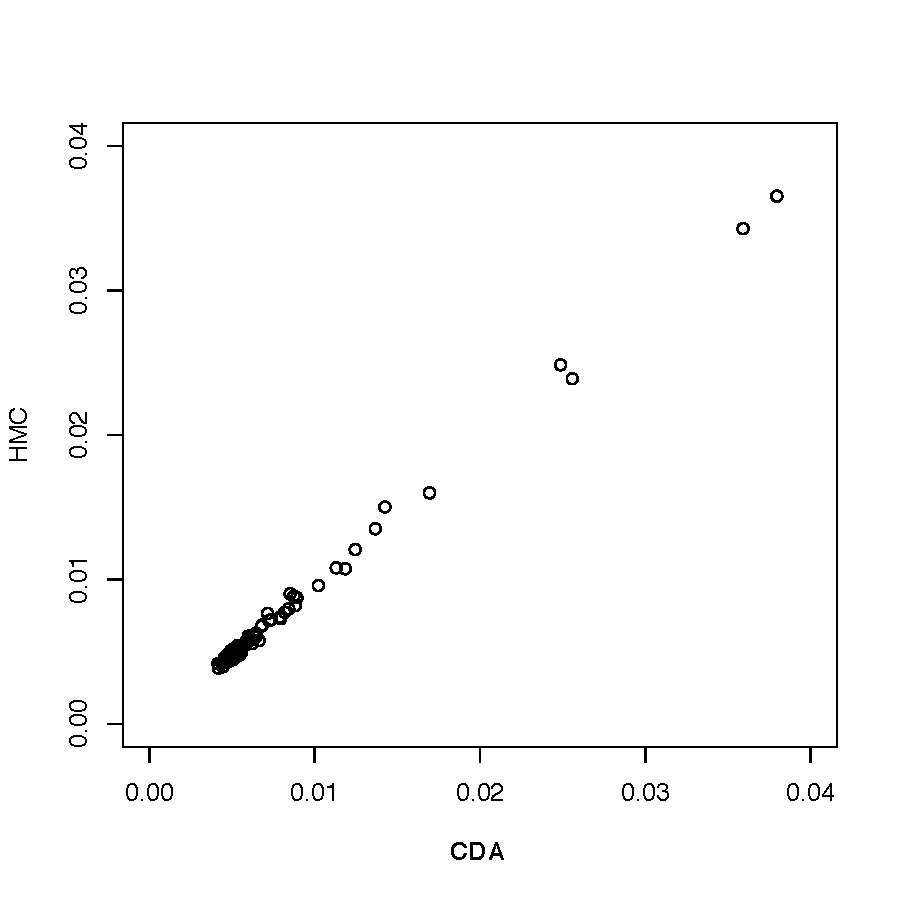
\includegraphics[width=1\textwidth]{CDAvsHMC_sd.pdf}
 \caption{Comparing posterior standard deviation for $\beta_1,\dots \beta_{95}$ from the HMC and CDA.}
 \end{subfigure}  
 \caption{The results from CDA and HMC agree very well.}
 \end{figure}

\subsection{Mixing of HMC}


 \begin{figure}[H]
 % \centering
   \begin{subfigure}[b]{0.45\textwidth}
 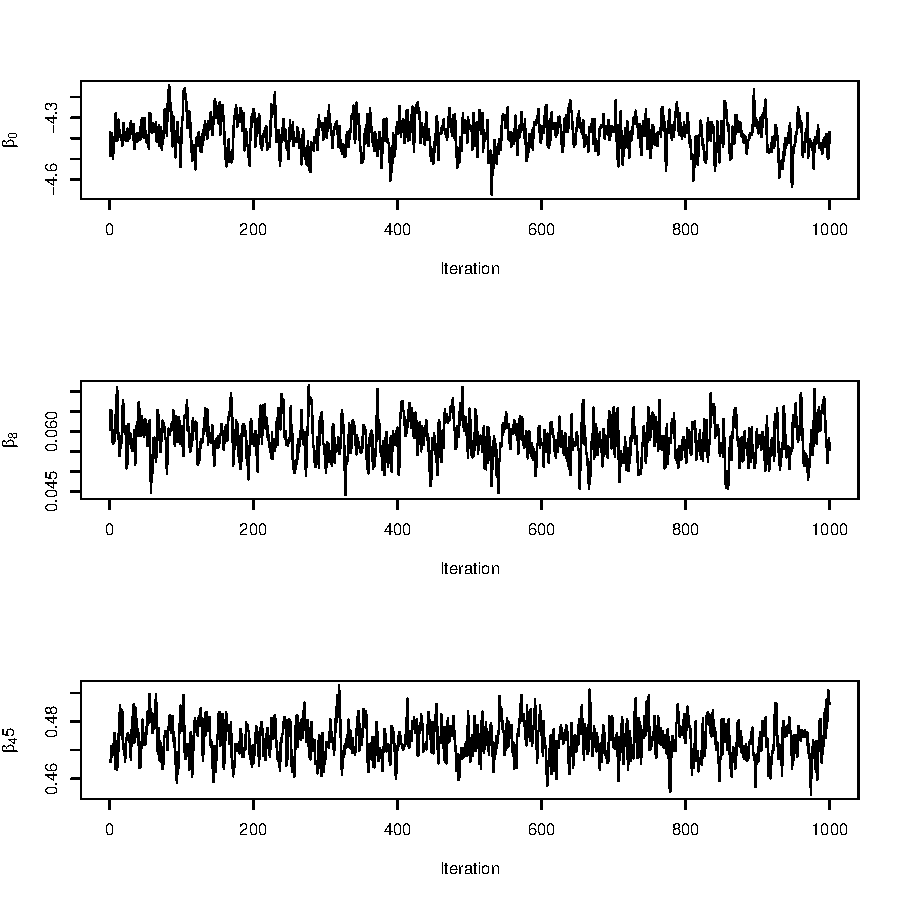
\includegraphics[width=1\textwidth]{traceplot_poisson_ada.pdf}
 \caption{Traceplots}
 \end{subfigure}
  \hfill 
 \begin{subfigure}[b]{0.45\textwidth}
 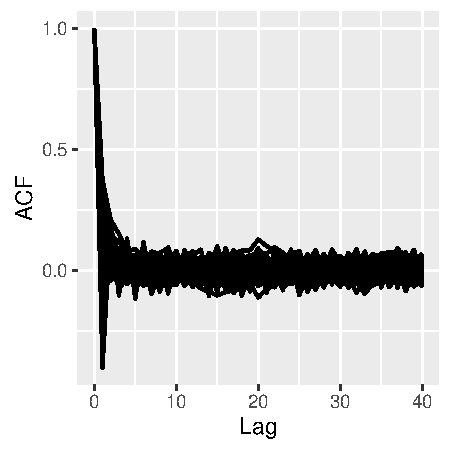
\includegraphics[width=1\textwidth]{poisson_hmc_acf.pdf}
 \caption{Autocorrelation}
 \end{subfigure}  
 \caption{The posterior estimates produced by HMC.}
 \end{figure}
 


 
\end{document}




